\PassOptionsToPackage{intlimits}{amsmath}
\documentclass[journal]{IEEEtran}
\usepackage{catchfilebetweentags}
\newcommand{\loadeqn}[1]{%
    \ExecuteMetaData[equations.tex]{eq#1}%
}
\newcommand{\loadfig}[1]{%
    \ExecuteMetaData[figures.tex]{fig#1}%
}
\usepackage[margin=0.7in]{geometry}
\usepackage[parfill]{parskip}
\usepackage[backend=biber, bibencoding=utf8, style=ieee, backref=true]{biblatex}
\usepackage[hyperfootnotes=false,hyperindex=true]{hyperref}
\usepackage[utf8]{inputenc}
\usepackage{amsmath,amssymb,amsfonts,amsthm} % math
\usepackage{bm} % \bm 
\usepackage{physics} % \pdv
\usepackage{mathtools} % coloneqq
\usepackage{imakeidx} % index
\usepackage{etoc} % localtabelofcontents
\usepackage{tikz}
\usetikzlibrary{}

\usepackage{pgfplots}
\usepackage{subcaption}
\DeclareCaptionFormat{subfig}{#1#2#3}
\DeclareCaptionSubType{figure}
\captionsetup[subfigure]{format=subfig,labelsep=space,labelformat=parens}


\newcommand{\newterm}[1]{\textit{#1}\index{#1}}
\newcommand{\Xk}{X_k}
\newcommand{\Xkone}{X_{k+1}}
\newcommand{\bx}{\bm{x}}
\newcommand{\bX}{\bm{X}}
\newcommand{\bxi}{\bm{x}_i}
\newcommand{\delx}{\bx - \bxi}
\newcommand{\by}{\bm{y}}
\newcommand{\bY}{\bm{Y}}
\newcommand{\byi}{\bm{y}_i}
\newcommand{\dely}{\by - \byi}
\newcommand{\zbx}{Z(\bx)}
\newcommand{\zbxi}{Z(\bxi)}
\newcommand{\bb}{\bm{\beta}}
\newcommand{\hzbx}{\hat{Z}(\bx)}
\NewDocumentCommand{\evalat}{sO{\big}mm}{%
  \IfBooleanTF{#1}
   {\mleft. #3 \mright|_{#4}}
   {#3#2|_{#4}}%
}
\theoremstyle{definition}
\newtheorem{theorem}{Theorem}[section]
\theoremstyle{definition}
\newtheorem{example}{Example}[section]


\makeindex
%! Suppress = GatherEquations
% introduction
\anotecontent{hom}{
If \(A\) and \(B\) are modules over a ring \(R\), then \(\operatorname{Hom}_R(A,B)\) is the set of all \(R\)-module homomorphisms \(f\colon A \rightarrow B\). In this case \(V\) is a module over \(\R\) and \(\R\) is trivially a module over \(\R\). 
}
\anotecontent{alternating}{An alternating function is one that changes signs if arguments are transposed (e.g. cross-product or determinant).}

\begin{document}
\title{Super Resolution for Automated Target Recognition}
\author{Maksim Levental}
\maketitle

\begin{abstract}
	Super resolution is the process of producing high-resolution images from low-resolution images while preserving ground truth about the subject matter of the images and potentially inferring more such truth.
	%
	Algorithms that successfully carry out such a process are broadly useful in all circumstances where high-resolution imagery is either difficult or impossible to obtain.
	%
	In particular we look towards super resolving images collected using longwave infrared cameras since high resolution sensors for such cameras do not currently exist.
	%
	We present an exposition of motivations and concepts of super resolution in general, and current techniques, with a qualitative comparison of such techniques.
	%
	Finally we suggest directions for future research.
\end{abstract}
% \newpage
\tableofcontents

% \newpage
Super-resolution (SR) is a collection of methods\anote{vbsuper} that augment the resolving power of an imaging system.
%
Here, and in the forthcoming, by resolving power we mean the ability of an imaging device to distinguish distinct but proximal objects in the scene.
%
If such objects are modeled as point sources of light then the resolving power of the imaging system is defined by Rayleigh's criterion: two point sources are considered \textit{resolved} when the first diffraction maximum\anote{rayleighscriterion} of one point source (at most) coincides with the first minimum of the other (see figure~\ref{fig:rayleigh}).
\begin{figure}
    \center
    \includegraphics[width=.5\linewidth]{figures/rayleigh.png}
    \caption{Rayleigh's criterion\cite{rayleigh}}
    \label{fig:rayleigh}
\end{figure}

SR techniques yield high-resolution (HR) images from one or more observed low-resolution (LR) images by restoring lost fine details and reversing degradations produced by imperfect imaging systems.
%
In the case when a single LR source image is used to construct the HR correspondent, the techniques are referred to as single-image-super-resolution (SISR) techniques.
%
These techniques typically operate by either learning some mapping from low resolution chips (uniform partitions of the image, e.g. $3\times 3$ pixels) to higher resolution chips that are highly similar (according to some metrics) and which obey regularity constraints (e.g. agreement at edges).
%
In the case when multiple LR source images are used to construct the single HR correspondent, the techniques are referred to as multiple-image-super-resolution (MISR) techniques.
%
MISR techniques rely on non-redundant and yet pertinent information in multiple images of the same scene (see figure~\ref{fig:misr}).
\begin{figure}
    \includegraphics[width=\linewidth,keepaspectratio]{figures/misr.png}
    \caption{Multiple image super resolution\cite{misr}}
    \label{fig:misr}
\end{figure}
%
Note that for such information to exist there should be sub-pixel\anote{subpixel} shifts in either the imaging system or the scene between consecutive images.


For typical imaging use-cases, high resolution images are preferable to low resolution images; higher resolutions are
desirable in and of themselves and as inputs to later image processing transformations that can degrade image quality (e.g.\ by virtue of quantization or compression).
%
In theory the resolving power of an imaging system is primarily determined by the number of independent sensor elements that comprise that imaging system (each of which collects a component of the ultimate image).
%
Naturally then, a way to increase the resolution of such a system is to increase the density of such sensor elements per unit area.
%
Unfortunately, and counter-intuitively, since the number of photons incident on each sensor decreases as the sensor shrinks, shot noise\anote{shotnoise} thwarts that idea.
%
Furthermore, while sensor density is primary, secondary effects due to optics limit resolution as well;
the point spread of a lens (distortion of a point source due to diffraction), chromatic aberrations (distortion due to differing indices of refraction for differing wavelengths of light), and motion blur all function to obscure or erase details from the image.


In domains such as satellite/aerial photography, medical imaging, and facial recognition,
high-resolution reconstruction of low-resolution samples is eminently useful since ab-initio acquisition of high-resolution images is either logistically difficult or impossible due to aforementioned imaging apparatus limitations.
%
For example in the instance of satellite imagery, acquisition of high-resolution imagery is primarily hampered by optics and physics\anote{satelliteoptics}.
%
In contrast, in the cases of medical imaging (where procedures are invasive and patient exposure time needs to be minimized\cite{doi:10.1002.cmr.a.21249}) and facial recognition (e.g.\ for purposes of surveillance) the primary challenge is logistics and access to repeat collection opportunities.


The benefits of enhancing images using SR techniques include not only more pleasing or more readily interpretable images for human consumption but higher quality inputs for automated learning systems as well.
%
In particular object detection systems trained on super-resolved images outperform those trained on the low
resolution originals\cite{effectssuperres}.
%
Indeed this is our ultimate goal - not super-resolution per se but super-resolution in the service of improved object detection performance for longwave-infrared (LWIR) imagery.
%
Note that while practically speaking, there exist hardware and software solutions for increasing the resolution of an imaging
system, we, owing to a "Ship of Theseus" consideration, discount such propositions.
%
We instead take low resolution images as given and seek techniques that allow for ex post facto reconstruction or inference of precise details.
%
This necessarily constrains techniques under consideration to be algorithmic in nature and software in practice.

The rest of this survey is outlined as follows: Section~\ref{sec:background} introduces imaging systems, notation, and the model of imaging that will be the mathematical framework for the proceeding sections, Section~\ref{sec:classical-algorithms} surveys classical techniques (those that do not employ neural networks), Section~\ref{sec:deep-learning-algorithms} surveys neural-network techniques with heavy emphasis on deep learning (i.e.\ deep networks), Section~\ref{sec:future-research} discusses the scope and goals of the author's research program, and Section~\ref{sec:conclusion} summarizes.


\newpage
\section{Background}\label{sec:background}
\localtableofcontents
\subsection{Imaging systems}\label{subsec:imaging-systems}
\begin{figure}[!htbp]
	\includegraphics[width=\linewidth,keepaspectratio]{figures/background/bccd.png}
	\caption{CCD buried channel MOS capacitor \cite{finaltestguideline}.}
	\label{fig:mos-cap}
\end{figure}

We begin with a practical discussion of imaging systems.
%
An imaging system consists of an imaging sensor and optics. 
%
An imaging sensor is a device that converts an optical image into a digital signal.
%
Charge-coupled devices (CCD) and complementary metal-oxide-semiconductor (CMOS) devices are the most common imaging sensors; CCDs have better performance while CMOS devices are newer and less expensive.
%
A third type that's of particular interest to us is the microbolometer, which is used as a sensor in thermal cameras.

\subsubsection{CCD Devices}

CCDs consist of two components: an imaging component and a readout component.
%
The imaging component is arranged with every third stripe of electrode tied electrically to form three sets of equipotentials.
%
These equipotentials taken together constitute a \textit{vertical register} (VR) (see figure~\ref{fig:ccd-array}).
\begin{figure*}[!htbp]
	\centering
	\includegraphics[width=.8\textwidth,keepaspectratio]{figures/background/ccd_array.png}
	\caption{CCD array with both image and readout components \cite{pawley1995handbook}. Note that all electrodes intersecting \(\Phi i\) for some \(i\) are at the same potential (voltage).}
	\label{fig:ccd-array}
\end{figure*}
%
A vertical register moves the collected photoelectrons down one electrode line at a time, using charge coupling, with the aid of channel stops (which function to prevent diffusion of charge across channels).

More precisely the imaging component of a CCD consists of densely packed two-dimensional arrays of buried channel\anote{buriedchannel} metal-oxide-semiconductor (MOS) capacitors (see figure~\ref{fig:mos-cap}).
%
Individual MOS capacitors are biased by a gate voltage such that a potential well develops in the n-type\anote{ntype} silicon.
%
This potential well acts as a storage system for charge induced by the inner photoelectric effect\anote{innerphotoelectric}.
%
When photons are incident on a MOS capacitor some of the photons are absorbed at the surface, some are scattered at the surface, and some are transmitted into the bulk material.
%
Those photons that are transmitted interact with electrons in the valence band of the silicon substrate and thereby excite them into the semiconductor's conduction band.
%
This creates electron-hole pairs that either diffuse or recombine (in the silicon).
%
For high-quality silicon, the lifetime of such a pair is several milliseconds (before recombination) \cite{scientificccd}.
%
The electrons of the electron-hole pairs (that do not recombine) then diffuse into the potential well, while the holes migrate to the grounded substrate (i.e., out of the sensor).
%
Electrons created in this way are called \textit{photoelectrons}.

Suppose the VR is in a state such that there's a collection of photoelectrons on each channel at equipotential \(\Phi1\) and only \(\Phi1\). Note this means \(\Phi2, \Phi3\) are at \(0\)v (again just as in figure~\ref{fig:mos-cap}). The VR mechanism that shifts collected charge operates as follows:
\begin{framed}
\begin{enumerate}
	\item \(\Phi2\) is positively biased to \(10\)V. This causes redistribution of charge such that it is diffused underneath both \(\Phi1\) and \(\Phi2\).
	\item \(\Phi1\) is set to \(0\)v. This concentrates the charge exclusively under \(\Phi2\).
	\item The same redistribution is repeated vis-à-vis \(\Phi2, \Phi3\) and \(\Phi3, \Phi1\).
	\item The entire process repeats thereby shifting the charge three electrode lines (or one pixel row) at a time.
	\item At the bottom of the image section \(\Phi3\) transfers all charge to the horizontal register which functions much like the VR except faster.
\end{enumerate}
\end{framed}
%
An obvious challenge faced by this system is how to prevent errant charge from accumulating out of sync with the shift process, i.e., how to prevent new photoelectrons from being produced at intermediate electrode lines while far lines are being shifted.
%
The solution is to have interstitial dedicated shift channels in between columns of sensors, with the shift channels being masked off from exposure to light.
%
This type of reading is called \textit{interline transfer} because the accumulated charge is first moved one line over, into the shift channels.
%
Naturally, interline transfer shrinks photosensitive area by half and despite possible solutions (e.g, micro-lenses being used to focus most of the light onto the unmasked sensors) this is one of the drawbacks of CCDs relative to CMOS devices.

\subsubsection{CMOS Devices}

CMOS devices consist of arrays of photodiodes (see figure~\ref{fig:photodiode.png}).
\begin{figure}[!htbp]
    \centering
    \begin{subfigure}[b]{0.49\textwidth}
        \includegraphics[width=\linewidth,keepaspectratio]{figures/background/cmos/photodiode.png}
        \caption{Photodiode schematic. L\textsubscript{e}, L\textsubscript{h} are electron, hole diffusion lengths respectively \cite{Xu2015FundamentalCO}.}
        \label{fig:photodiode.png}
    \end{subfigure}
    \vskip\baselineskip
    \begin{subfigure}[b]{0.49\textwidth}
        \center
        \includegraphics[width=.8\linewidth,keepaspectratio]{figures/background/cmos/3t_pixel.png}
        \caption{Three transistor pixel. M\textsubscript{rst} is the reset transistor (enabling the photodiode to dump charge), M\textsubscript{sf} buffers the charge on the photodiode (so that it can be read without loss), and M\textsubscript{sel} enables a whole row of pixels to be read simultaneously (since all pixels in a physical row are tied to the same row line).}
        \label{fig:3tpixel}
    \end{subfigure}
    \caption{CMOS components.}
\end{figure}
A photodiode is a \textit{p-n junction}\anote{pnjunction} operated in reverse bias mode\anote{reversebias}.
%
When a photon of sufficient energy is absorbed by the diode, it creates an electron-hole pair (as a result of the photoelectron effect).
%
If the creation event happens within the active region then the hole migrates out through the p-type material and the electron migrates out through the n-type material.
%
This establishes a \textit{photocurrent} that can be interrogated by a reading circuit (see figure~\ref{fig:3tpixel}).

CMOS sensor arrays do not shift the charge from row to row like CCD arrays.
%
In a CMOS sensor array, each pixel contains a transistor M\textsubscript{sel} controlled by the voltage applied across a row (see figure~\ref{fig:cmosarray}).
%
In order to read one row of pixels, a rowline is raised high to turn on (close) all the M\textsubscript{sel} transistors in the row.
%
This brings the signals from all the pixels in that row to the shift register below by way of the column lines.
%
The shift register then outputs the values of the pixels.

The high number of transistors needed per pixel in CMOS arrays has only recently become feasible for semiconductor foundries to manufacture.
%
This, along with such artifacts as the rolling shutter effect produced by rowline reading, are some of the drawbacks of CMOS devices relative to CCD devices.
%
Despite this CMOS devices have become the most common imaging system in consumer goods such as cell phones and digital cameras due to their relatively simple mechanics.
\begin{figure}[!htbp]
	\center
	\includegraphics[width=.8\linewidth,keepaspectratio]{figures/background/cmos.png}
	\caption{CMOS array of red, green, and blue pixels.}
	\label{fig:cmosarray}
\end{figure}

\subsubsection{Microbolometers}

Despite their ubiquity in visible spectrum devices, neither CCD arrays nor CMOS arrays can be adapted to capture any portion of the infrared spectrum.
%
A microbolometer, on the other hand, measures the power in the infrared by exposing a thermistor\anote{thermistor} to the incident light.
%
\begin{figure}[!htbp]
	\center
	\includegraphics[width=\linewidth,keepaspectratio]{figures/background/microbolometer2.png}
	\caption{Bridge structure of Honeywell microbolometer \cite{KESIM2014245}.}
	\label{fig:microbolometer}
\end{figure}
%
Since a thermistor's resistance changes as a function of its temperature, a key issue in the design of a microbolometer is the thermal isolation of the thermistor.
%
With the maturation of micro-machining techniques (such as for MEMS\anote{mems} devices) over the last few years efficient microbolometers have become possible.
%
There are now many consumer thermal cameras on the consumer market powered by two-level microbolometer pixels consisting of a thermo-sensitive component suspended above (and insulated from) silicon (see figure~\ref{fig:microbolometer}).

These pixel packages are evacuated in order that they have good conduction, convection, and radiation heat transfer properties.
%
The actual thermo-sensitive component consists of a thermistor, an absorber (which aids in the transfer of heat to the thermistor), and a reflector that creates a Fabry–Pérot optical cavity\anote{fabryperot} (typically \({\sim}\lambda/4\) \cite{bolometer}) that traps the infrared light.
%
Typical materials for the thermistor are vanadium oxide and amorphous silicon owing to their high temperature coefficients of resistance \cite{bolometer}, which, in effect transform small changes in temperature into large changes in resistance.
%
Measurements of the thermistor are performed by a read-out integrated circuit adjacent to the bridge in the silicon substrate.
%
It is plain to see that microbolometers are designed much differently from either CCD or CMOS arrays.
%
As a result of this fact, high-resolution infrared imaging systems are not as of yet available on the consumer market and hence our interest in applying super-resolution to images collected by such systems.
%
With that in mind, we now proceed to formalizing the problem of super-resolution.

\subsection{Interlude: Mathematical Notation}\label{subsec:notation}

Upper case plain latin \(X, Y\) each denote channel \(\times\) row \(\times\) column \textit{tensors}\anote{tensor} representing LR and HR images respectively, with \((0, 0,0)\) corresponding to the top left corner of the first channel of image.
%
Often for the sake of simplicity we consider grayscale images, in which case we omit the channel dimension.
%
\(D, H, F, G\) variously refer to functions that operate on images.
%
Bolded uppercase latin are reserved for batches of objects.
%
For example \(\bm{X}, \bm{Y}\) are batches of images, i.e., batch size \(\times\) channel \(\times\) row \(\times\) column tensors with \((0, 0, 0,0)\) corresponding to the top left corner of the first channel of first image in the batch.
%
Bolded lower case latin such as \(\bm{x}, \bm{y}, \bm{z}\) denotes a conventional column or row vector.
%
Subscripts are used most often to indicate sequences (e.g., \(X_1, X_2, \dots\)) but occasionally indicate position (e.g., \((U_x, U_y)\)).
%
The \(L_2\) norm is indicated by unadorned \(\abs{\cdot}\).
%
All other norms are indicated by a subscript (e.g. \(\abs{\cdot}_1\) is the \(L_1\) norm).
%
New mathematical quantities are defined on first use by colon-equals \(\coloneqq\).
%
Hats denote computed estimators (e.g., \(\hat{X}\) is an estimate of \(X\) given noisy samples \(X_i\)).
%
All other notation is defined in situ.

\subsection{Imaging model}\label{subsec:imaging-model}

Figure~\ref{fig:bertrand} shows a conceptual model of the imaging process as carried out by an imaging system.
%
The input to the system is a natural scene that is in effect sampled by the imaging system.
%
In the idealized case, the sampling is done at (or above) the Nyquist rate and no aliasing occurs.
%
In practice there is noise and loss introduced at every step of the process: atmospheric turbulence plays a role at large distances, motion produces multiple views of the same scene but also induces blur, imperfections of the lenses further blur the image, and finally down-sampling by the sensor elements into pixels produces aliasing artifacts\anote{ccd}.
%
The noisy, blurry, down-sampled images are then further degraded by sensor noise.
%
Each such image we call an LR sample.
\begin{figure*}
	\centering
	\begin{adjustbox}{width=\textwidth}
		\begin{tikzpicture}[auto]
			\tikzstyle{terminal} = [rectangle, draw, text width=5em, text centered, minimum height=4em]
			\tikzstyle{block} = [rectangle, draw, fill=gray!20, text width=6em, text centered, rounded corners, minimum height=4em]
			\tikzstyle{line} = [draw, -latex']
			\tikzstyle{sum} = [circle, draw]

			\node[inner sep=0pt] (bertrand) {\includegraphics[width=.15\textwidth]{figures/bertrand/bertrand.png}};
			\node [above = of bertrand] (scene) {Scene};

			\node[sum, right = of bertrand] (sum1) {$+$};
			\node [block, below = of sum1] (atmo-noise) {Atmospheric noise};

			\node [block, right = of sum1] (motion) {Translation, Rotation, Aspect};
			\node [above = of motion] {Motion};

			\node [inner sep=0pt, right = of motion] (motion-output) {};

			\node[inner sep=0pt, below = of motion-output] (bertrand-motion) {\includegraphics[width=.15\textwidth]{figures/bertrand/bertrand.png}};
			\node[inner sep=0pt, below = of motion-output, xshift=2mm, yshift=-2mm] {\includegraphics[width=.15\textwidth]{figures/bertrand/bertrand.png}};
			\node[inner sep=0pt, below = of motion-output, xshift=4mm, yshift=-4mm] {\includegraphics[width=.15\textwidth]{figures/bertrand/bertrand.png}};
			\node[inner sep=0pt, below = of motion-output, xshift=6mm, yshift=-6mm] {\includegraphics[width=.15\textwidth]{figures/bertrand/bertrand.png}};

			\node [block, right = of motion-output] (blur) {Optical, Motion};
			\node [above = of blur] {Blur};
			\node [inner sep=0pt, right = of blur] (blur-output) {};

			\node[inner sep=0pt, below = of blur-output] (bertrand-blur) {\includegraphics[width=.15\textwidth]{figures/bertrand/bertrand-blur.png}};
			\node[inner sep=0pt, below = of blur-output, xshift=2mm, yshift=-2mm] {\includegraphics[width=.15\textwidth]{figures/bertrand/bertrand-blur.png}};
			\node[inner sep=0pt, below = of blur-output, xshift=4mm, yshift=-4mm] {\includegraphics[width=.15\textwidth]{figures/bertrand/bertrand-blur.png}};
			\node[inner sep=0pt, below = of blur-output, xshift=6mm, yshift=-6mm] {\includegraphics[width=.15\textwidth]{figures/bertrand/bertrand-blur.png}};

			\node[block, right = of blur-output] (downsample) {Quantization, Pixel-binning};
			\node [above = of downsample] {Down-sampling};

			\node[sum, right = of downsample] (sum2) {$+$};
			\node [block, below = of sum2] (sensor-noise) {Sensor noise};

			\node[inner sep=0pt, right = of sum2] (bertrand-blur-noise) {\includegraphics[width=.1\textwidth]{figures/bertrand/bertrand-blur-noise.png}};
			\node[inner sep=0pt, right = of sum2, xshift=2mm, yshift=-2mm] {\includegraphics[width=.1\textwidth]{figures/bertrand/bertrand-blur-noise.png}};
			\node[inner sep=0pt, right = of sum2, xshift=4mm, yshift=-4mm] {\includegraphics[width=.1\textwidth]{figures/bertrand/bertrand-blur-noise.png}};
			\node[inner sep=0pt, right = of sum2, xshift=6mm, yshift=-6mm] {\includegraphics[width=.1\textwidth]{figures/bertrand/bertrand-blur-noise.png}};
			\node [above = of bertrand-blur-noise, text width=5em] (lr-output) {Low-resolution images};

			\draw[-] (bertrand) edge (sum1);
			\draw[->] (sum1) edge (motion);
			\draw[->] (atmo-noise) edge (sum1);

			\draw[->] (motion) edge (blur);
			\draw[->] (motion-output) edge (bertrand-motion);

			\draw[->] (blur) edge (downsample);
			\draw[->] (blur-output) edge (bertrand-blur);
			\draw[->] (sensor-noise) edge (sum2);
			\draw[-] (downsample) edge (sum2);
			\draw[->] (sum2) edge (bertrand-blur-noise);
		\end{tikzpicture}
	\end{adjustbox}
	\caption{The imaging model illustrating the relationship between a scene and final low-resolution images due to noise, motion, blur, and sampling.}
	\label{fig:bertrand}
\end{figure*}

Let \(Y\) denote an idealized HR image of the scene from some fixed vantage point and assume the imaging system collects \(K\) LR samples \(\Xk\) of \(Y\).
%
Formally the \(\Xk\) are related to \(Y\) by
\begin{equation}
	\Xk = (D \circ H_k \circ A_k) (Y) + \varepsilon_k
	\label{eqn:imagingmodel}
\end{equation}
where for the \(k\)th LR sample, \(A_k\) (of \(K\)) is the operator representing motion, \(H_k\) represents the blur operator, \(D\) represents the down-sampling operator (constant in time since it's typically a digital component of the imaging system), and \(\varepsilon_k\) represents the composite noise (environment and sensor noise).

\subsubsection{Motion}

In the case of MISR, high-resolution images are constructed by exploiting distinct scene data among multiple low-resolution images.
%
Such distinct data are produced by the relative motion of the imaging system and the scene and therefore precise and accurate image \textit{registration}\anote{registration} is paramount.
%
Successful registration is effected by producing a transformation \(f\) that maps pixels at coordinates \((x',y')\) in sample \(\Xkone\) to coordinates \((x,y)\) in sample \(X_j\)
\begin{equation}
	\Xkone(f(x', y')) = X_j(x,y)
	\label{eqn:registration}
\end{equation}
where we use index \(j\) to indicate the possibility of registering all samples relative to a fixed reference image (e.g. \(j=0\) the first sample) or successive/relative registration (i.e.,with \(j=k\)).
%
While image registration is already challenging in the various domains where samples are treated as canonical, such as remote sensing and medical imaging, in SR it is further complicated by the fact that the images to be registered are assumed uncertain.
%
Therefore, in principle, image registration and super-resolution cannot be decoupled, since image registration accuracy would be improved by operating on the estimated HR images;
%
Hardie \etal \cite{Hardie1997} use a Bayesian framework to jointly estimate image registration parameters and the high-resolution image \cite{Hardie1997}.
%
Alternatively one can marginalize over the HR image and estimate the registration parameters using maximum-likelihood estimation (MLE) (see section~\ref{subsubsec:gaussianprocess}).

\subsubsection{Blur}

We now consider the challenges and nuances of estimating blur.
%
In general, the optical transfer function (OTF) characterizes the blur of an imaging system\anote{otf}.
%
We factor the OTF into three components:
\begin{equation}
	H(u, v) \coloneqq H_{\text{diff}}(u,v) H_{\text{abr}}(u,v) H_{\text{int}} (u,v)
\end{equation}
where \(u,v\) are horizontal and vertical spatial frequencies respectively (measured in cycles/mm), \(H_{\text{diff}}\) is blur due to diffraction, \(H_{\text{abr}}\) is blur due to lens aberrations, and \(H_{\text{int}}\) is blur due to imaging sensor shape (obtained by taking the Fourier transform of the shape an individual sensor in the imaging array).
%
Blur due to diffraction in most imaging systems is due to diffraction through a circular aperture \cite{goodman2005introduction}:
\begin{equation*}
	H_{\text{diff}}(u,v) =   \begin{cases}
		\frac{2}{\pi} \left(\frac{1}{\cos(\tau)} - \tau \sqrt{1-\tau^2}\right) & \text{if } \tau < 0 \\
		0                                                                      & \text{otherwise}
	\end{cases}
\end{equation*}
where \(\tau = \rho/\rho_c\), \(\rho=\sqrt{u^2 +v^2}\), \(\rho_c = 1/\lambda N\) is the radial cutoff frequency of the aperture, \(N\) is the f-number\anote{fnumber} of the optics, and \(\lambda\) is the wavelength of light being diffracted.
%
This is in fact the filter that produces the Airy pattern and therefore informs sensor array spacing in order to avoid aliasing.
%
Wavelength independent blurring due to aberrations can be induced by various imperfections in the lenses such as spherical aberration, comatic aberration\anote{coma}, or astigmatism. Furthermore, dispersion\anote{dispersion} blurs particular wavelengths of light. A good model for all of these effects is \cite{10.1117.12.946501}:
\begin{equation*}
	H_{\text{abr}}(u,v) =   \begin{cases}
		1-\left(\frac{25}{65}\right)^2 \left(1-4\left(\tau - \frac{1}{2}\right)\right)^2 & \text{if } \tau < 0 \\
		0                                                                                & \text{otherwise}
	\end{cases}
\end{equation*}
Figure~\ref{fig:mtf} shows an example OTF for an imaging system with a sensor spacing of 0.050 mm and therefore sampling frequency of 20 cycles/mm and \(\rho_c = 83.3~\text{cycles}/\text{mm}\) (\(F=3\) and \(\lambda = 4\mu\text{m}\) i.e.,near infrared).
%
Notice that \(\rho_c\) is much greater than the Nyquist rate (\(\frac{1}{2} \times 20~\text{cycles}/\text{mm} = 10~\text{cycles}/\text{mm}\)) and therefore many frequencies that are within the radial cutoff frequency will be aliased.
%
This in particular can be mitigated by effectively increasing sampling rate using MISR.
%
Notice also that like a typical transfer function the OTF is not flat and therefore attenuates high spatial frequencies.
%
Simply applying gain to the image wouldn't solve the attenuation problems because of aliasing, but likewise this can be resolved after the effective sampling rate is increased using MISR.
\begin{figure}[!htbp]
	\includegraphics[width=\linewidth,keepaspectratio]{figures/background/mtf.png}
	\caption{OTF magnitude cross-section for \cite{milanfar2017super}.}
	\label{fig:mtf}
\end{figure}

The challenge of super-resolution is to solve the inverse problem of finding \(Y\) from one or several \(\Xk\).
%
In general, since \(A_k, H_k, D_k\) are highly degenerate functions, the corresponding inverse problems are ill-posed without regularization and conditioning.
%
The techniques that have been brought to bear on the problem range from interpolation to statistical estimation to example based learning.


\newpage
\begin{figure*}
    \begin{tikzpicture}[scale=1,every node/.style={minimum size=1cm},on grid]
        \tikzstyle{diff} = [draw, circle, scale=0.5]
        \foreach \Sigma in {0,...,4} {
            \node[yshift=-350+\Sigma*30, yslant=0.5, xslant=-1.5, scale=1] (bertrand-blur-\Sigma-1) {
                \includegraphics[width=.15\textwidth]{figures/sift/bertrand_sigma_1_\Sigma.png}
            };

        }
        \foreach \Sigma in {0,...,4} {
            \node[yshift=-150+\Sigma*20, xshift=30, yslant=0.5, xslant=-1.5, scale=0.5] (bertrand-blur-\Sigma-2) {
                \includegraphics[width=.15\textwidth]{figures/sift/bertrand_sigma_1_\Sigma.png}
            };
        }
        \foreach \Sigma in {0,...,4} {
            \node[yshift=-10+\Sigma*20, yslant=0.5, xshift=30, xslant=-1.5, scale=0.25] (bertrand-blur-\Sigma-3) {
                \includegraphics[width=.15\textwidth]{figures/sift/bertrand_sigma_1_\Sigma.png}
            };
        }

        \foreach \Sigma in {1,...,4} {
            \begin{scope}[
               yshift=-365+\Sigma*30, xshift=280,every node/.append style={
               yslant=0.5, xslant=-1.5},yslant=0.5, xslant=-1.5
           ]
               \node[] (bertrand-dog-\Sigma-1) {
                    \includegraphics[width=.15\textwidth]{figures/sift/dog_bertrand_sigma_1_\Sigma.png}
                };
               \fill[green] (2.05,2.05) rectangle (2.35,2.35); % center pixel
               \fill[green] (1.65,2.05) rectangle (1.95,2.35); %left
               \fill[green] (2.45,2.05) rectangle (2.75,2.35); %right
               \fill[green] (2.05,2.45) rectangle (2.35,2.75); %top
               \fill[green] (2.05,1.95) rectangle (2.35,1.65); %bottom
            \end{scope}

%            \node[] (bertrand-dog-\Sigma-1) {
%                \includegraphics[width=.15\textwidth]{figures/sift/dog_bertrand_sigma_1_\Sigma.png}
%            };
           \draw[yshift=-365+\Sigma*30, xshift=280, step=1mm, black, yslant=0.5, xslant=-1.5] (-1,-1) grid (0,0);
           \draw[yshift=-365+\Sigma*30, xshift=280, black,thick, yslant=0.5, xslant=-1.5] (-1,-1) rectangle (0,0);
        }
        \foreach \Sigma in {1,...,4} {
            \node[yshift=-365+\Sigma*30, xshift=140, diff] (diff-\Sigma-1){\Large$-$};
        }



        \foreach \Sigma in {1,...,4} {
            \node[yshift=-160+\Sigma*20, xshift=250, yslant=0.5, xslant=-1.5, scale=0.5] (bertrand-dog-\Sigma-2) {
                \includegraphics[width=.15\textwidth]{figures/sift/dog_bertrand_sigma_1_\Sigma.png}
            };
        }
        \foreach \Sigma in {1,...,4} {
            \node[yshift=-160+\Sigma*20, xshift=140, diff] (diff-\Sigma-2){\Large$-$};
        }



        \foreach \Sigma in {1,...,4} {
            \node[yshift=-5+\Sigma*20, xshift=250, yslant=0.5, xslant=-1.5, scale=0.25] (bertrand-dog-\Sigma-3) {
                \includegraphics[width=.15\textwidth]{figures/sift/dog_bertrand_sigma_1_\Sigma.png}
            };
        }
        \foreach \Sigma in {1,...,4} {
            \node[yshift=-5+\Sigma*20, xshift=140, diff] (diff-\Sigma-3){\Large$-$};
        }

        % draw annotations
        \foreach \x in {1,2,3} {
            \foreach \Sigma in {1,...,4} {
                \draw[-] (bertrand-blur-\Sigma-\x) edge (diff-\Sigma-\x);
            }
            \foreach \Sigma in {0,...,3} {
                \pgfmathtruncatemacro{\nodelabel}{1+\Sigma}
            \draw[-] (bertrand-blur-\Sigma-\x) edge (diff-\nodelabel-\x);
            }
            \foreach \Sigma in {1,...,4} {
                \draw[->] (diff-\Sigma-\x) edge (bertrand-dog-\Sigma-\x);
            }
        }


%           \fill[green] (2.05,2.05) rectangle (2.35,2.35); % center pixel
%           \fill[green] (1.65,2.05) rectangle (1.95,2.35); %left
%           \fill[green] (2.45,2.05) rectangle (2.75,2.35); %right
%           \fill[green] (2.05,2.45) rectangle (2.35,2.75); %top
%           \fill[green] (2.05,1.95) rectangle (2.35,1.65); %bottom
%    % 8 -pixel setting
%           \fill[green] (1.65,2.45) rectangle (1.95,2.75); %top-left
%           \fill[green] (2.45,2.45) rectangle (2.75,2.75); %top-right
%           \fill[green] (2.75,1.95) rectangle (2.45,1.65); %bottom-right
%           \fill[green] (1.65,1.95) rectangle (1.95,1.65); %bottom-left
%    % 2. ring
%           \fill[green] (1.25,1.55) rectangle (1.55,1.25); %bottom-left
%           \fill[green] (0.85,1.55) rectangle (1.15,1.25); %bottom-left
%           \fill[green] (0.85,1.15) rectangle (1.15,0.85); %bottom-left
%           \fill[green] (1.25,0.75) rectangle (1.55,0.45); %bottom-left


%    \draw[-latex,thick,blue](-3,5)node[left]{ }
%    to[out=0,in=90] (0.8,1.15);
%    \draw[-latex,thick,green](-3,5)node[left]{3 patches}
%    to[out=0,in=90] (0,2.8);
%    %
%    \draw[-latex,thick,green](-3,-2)node[left]{1 patch}
%    to[out=0,in=200] (-1,-.9);
%    \draw[thick,gray!70!black](6,4) node {4 neighbourhood rule};
%    \draw[thick,gray!70!black](6,-2) node {8 neighbourhood rule};
    %
    \end{tikzpicture}
%\end{adjustbox}
\caption{The imaging model illustrating the relationship between a scene and final low-resolution images due to noise, motion, blur, and sampling.}
\label{fig:bertrand}
\end{figure*}

Images obtained from multiple vantage points, or at different times, of the same scene, become distorted with respect
to each other.
%
Since in MISR the aim is to exploit new information across multiple LR samples we need to first rectify these distortions and reconcile the images.
%
Effectively this means finding one or more pixel transformations that enable mapping all LR images to a common pixel grid.
%
When the transformations cannot be deduced from first principles (e.g. precise knowledge of the relative motion of the scene and the imaging system) they must be estimated from the LR images.
%
There are broadly two perspectives on constructing the transformation \(f\) (see eqn.~\eqref{eqn:registration}): the global perspective which aims to model motion as a map of the image as a whole and the local perspective which aims to model motion as a deformation of individual pixels.
%
These two perspectives naturally correspond to a globally or locally defined transformation \(f\).
%
We first cover global algorithms, examining the different techniques available for each step, and then move on to local algorithms.

\subsection{Global Algorithms}

Most global image registration algorithms consist of a feature detection and selection step (also called Control Point (CP) selection), a feature matching step, and a transform estimation step.
%

\subsubsection{Feature Detection and Selection}

Feature detection and selection is the process of identifying features of the image that are presumed to be invariant across the multiple images to registered.
%
Note that here by features we mean image artifacts (e.g. edges, contours, line intersections, or corners); in this context encodings or transformations of these image artifacts are called \textit{descriptors}.
%
The CPs are the data that will be used to estimate the transformation \(f\).
%
Therefore, in order that the estimated transformation is accurate, CPs should be robust to noise and image degradation, sufficiently distributed throughout the image, and readily matched in the matching step.

\paragraph{Harris Corner Detection}
Bentoutou \etal\cite{bentoutou2005automatic} use a Harris detector\cite{harris1988combined} to find corner points, arguing that corners are robust to noise and stable over multiple images.
%
The Harris detector improves on the Moravec\cite{moravec1980obstacle} detector.
%
The Moravec detector starts from the error function \(E_{x,y}(u,v)\) which computes the sum of the squared differences (SSD) between an \(m \times m\) weighted window around a pixel \(X(x, y)\) and weighted windows shifted by \(u,v\) pixels:
\begin{multline}
    \quad E_{x,y}(u,v) \coloneqq \\ \sum_{i,j=-m/2}^{m/2} w_{ij}\left[ X(x_i+ u,y_j+v) - X(x_i, y_j)\right]^2
    \label{moravecerrorfunction}
\end{multline}
where \(x_i \coloneqq x + i\) and \(y_j \coloneqq y+j\).
\begin{figure}
    \centering
    \includegraphics[width=\linewidth,keepaspectratio]{figures/registration/corners.png}
    \caption{Moravec Corner Detector}
    \label{fig:corners}
\end{figure}
Moravec assigns a "corner score" according to the following reasoning (see figure~\ref{fig:corners}):
\begin{enumerate}
    \item If a pixel is in a region of uniform intensity then \(E_{x,y}(u,v)\) is small for all \(u,v\) (since neighboring windows are similar).
    \item If a pixel is on an edge, then \(E_{x,y}(u,v)\) for either \(u > 0\) or \(v > 0\), but not both, is high.
    \item If a pixel is on a corner, then \(E_{x,y}(u,v)\) for \(u > 0\) and \(v > 0\) is high.
\end{enumerate}
Therefore the corner score at pixel coordinate \((x,y)\) is \(\min_{u,v} E_{x,y}(u,v)\) in order to select for the third case.
%
Moravec comments that this corner score is not isotropic, i.e. if edges aren't aligned with either the pixel axes or diagonals then \(E_{x,y}(u,v)\) will incorrectly be low.
%
Harris' insight was to linearize \(E_{x,y}(u,v)\) in order to compute a quantity more closely related to the intensity variation in a local
neighborhood of a pixel:
\begin{equation}
    X(x_i + u,y_j + v) \approx  X(x_i,y_j) + \frac{\partial X}{\partial u}u + \frac{\partial X }{\partial v} v
\end{equation}
where the partial derivatives are taken at \((x,y)\).
%
This implies
\begin{align}
    E_{x,y}(u,v) & \approx \sum_{i,j=-m/2}^{m/2} w_{ij} \left[ X_u u + X_v v\right]^2                 \\
                 & = \sum_{i,j=-m/2}^{m/2} w_{ij} \left[ X_u^2 u^2 + X_v^2 v^2 + 2 X_u X_v u v\right] \\
                 & = \left[ u,v \right] \begin{bmatrix}
        \sum w_{ij}X_u^2   & \sum w_{ij}X_u X_v \\
        \sum w_{ij}X_u X_v & \sum w_{ij}X_v^2   \\
    \end{bmatrix}  \begin{bmatrix}
        u \\
        v
    \end{bmatrix}          \\
                 & = \left[ u,v \right] M  \begin{bmatrix}
        u \\
        v
    \end{bmatrix} \label{eqn:structurematrix}
\end{align}
where \(X_u = \partial X/\partial u\) and similarly \(X_v\).
%
The matrix in eqn.~\eqref{eqn:structurematrix}, called the \textit{structor tensor} or \textit{second-moment matrix} \(M\), is the quantity Harris investigated.
%
Harris reasoned that the cases of Moravec correspond to conditions on the eigenvalues \(\lambda_1, \lambda_2\) of \(M\):
\begin{enumerate}
    \item If \(\lambda_1 \approx \lambda_2 \approx 0\) then \(X(x,y)\) is in a region of uniform intensity.
    \item If \(\lambda_1 \gg \lambda_2\) or \(\lambda_2 \gg \lambda_1\) then \(X(x,y)\) is on an edge.
    \item \(\lambda_1 \approx \lambda_2 > 0\) then \(X(x,y)\) is on a corner.
\end{enumerate}
Notice that if \(w_{ij} = 1\) then this is just the gradient covariance of the image and the Harris detector is essentially a local Principle Components Analysis (PCA).
%
In fact Harris doesn't actually compute the eigenvalues but instead a related quantity called the "strength":
\begin{align}
    S & = \lambda_1 \lambda_2 - \kappa (\lambda_1 + \lambda_2)^2 \\
      & = \det(M) - \kappa \operatorname{trace}^2(M)
    \label{eqn:strength}
\end{align}
%
Hence Bentoutou \etal~first compute a gradient map of the image using a first order Gaussian derivative filter.
%
They then threshold\anote{threshold} the gradient map at the average gradient value, thereby extracting only sufficiently "interesting" regions, and compute the strength \(S\) for all pixels.
%
They also apply Non-maximum Suppression\anote{nms} (NMS) using a \(3 \times 3\) window and further threshold the remaining non-zero strength values at a threshold of 1\% of maximum observed strength.
%
Finally only the "strongest" \(n\) corners are kept.

\paragraph{SIFT}

\begin{figure}
    \centering
    \includegraphics[width=\linewidth,keepaspectratio]{figures/registration/sift/sift_scale_invariant.png}
    \caption{Harris Detector failing to recognize the right image as a corner.}
    \label{fig:sift_harris}
\end{figure}
One issue with Harris detectors is that they're not invariant to scale (see figure~\ref{fig:sift_harris}).
%
Zahra \etal\cite{zahrasift} resolves this issue by using the Scale Invariant Feature Transform\cite{lowe2004distinctive} (SIFT) to identify CPs that, as the name implies, are invariant across multiple scales.
%
SIFT identifies scale invariant and noise robust features of an image, called \textit{keypoints}, by first finding candidate points with high local curvature at multiple scales and then culling according to some heuristics.
\begin{figure*}
	\tikzstyle{every picture}+=[remember picture]
	\tikzset{
		pics/greensquare/.style args={#1/#2/#3}{
				code = {
						\draw[green] (#1,#2) rectangle (#1+#3, #2+#3);
					}
			},
		subgradbin/.pic={
				\foreach \i in {0.0, 1.0} {
						\pgfmathsetmacro{\x}{0.5+\i*2*.08825};
						\foreach \j in {0.0, 1.0} {
								\pgfmathsetmacro{\y}{0.5+\j*2*.08825};
								\pic[] {greensquare=\x/\y/2*.08825};
							}
					}
			},
		subgradbins/.pic={
				\foreach \x in {0,1,2,3} {
						\pgfmathtruncatemacro{\angle}{45+\x*90}
						\pic[rotate around={\angle:(0.5,0.5)}] {subgradbin};
					}
			},
		pics/edgehistogram/.style args={#1/#2}{
				code={
						\begin{axis}[area style, width=2.5cm,height=2.5cm, hide axis, at={(#1cm,#2cm)}]
							\addplot+[ybar interval] plot coordinates {
									(-0.50, 2) (0.5, 4) (1.5, 5) (2.5, 3) (3.5, 2) (4.5, 2) (5.5, 0)
								};
							\path
							\foreach[count=\i from 0] \v in {2, 4, 5, 3, 2, 2} {
									(\i, \v) node[below] {\tiny\v}
								};
						\end{axis}
					}
			},
		pics/randomedgehistogram/.style args={#1/#2}{
				code={
						\begin{axis}[area style, width=2.5cm,height=2.5cm, hide axis, at={(#1cm,#2cm)}]
							\pgfmathrandominteger{\na}{3}{4}
							\pgfmathrandominteger{\nb}{3}{4};
							\pgfmathrandominteger{\nc}{3}{8};
							\pgfmathrandominteger{\nd}{3}{8};
							\pgfmathrandominteger{\ne}{3}{4};
							\pgfmathrandominteger{\nf}{3}{4};
							\pgfmathrandominteger{\ng}{3}{4};
							\pgfmathrandominteger{\nh}{3}{4};
							\addplot+[ybar interval] plot coordinates {
									(-0.50, \na)
									(0.5, \nb)
									(1.5, \nc)
									(2.5, \nd)
									(3.5, \ne)
									(4.5, \nf)
									(5.5, \ng)
									(6.5, \nh)
									(7.5, 0)
								};
							\path
							\foreach[count=\i from 0] \v in {\na, \nb, \nc, \nd, \ne, \nf, \ng, \nh} {
									(\i, \v) node[below] {\scalebox{.3}{\v}}
								};
							\coordinate (hist-#1#2) at (5,-3);
						\end{axis}
					}
			},
		array/.style={draw, minimum width=2em, minimum height=2em,
				outer sep=0pt},
	}
	\newcommand*{\siftwidth}{.5\linewidth}
	\newcommand*{\length}{sqrt((2.*x^2+2.*y^2)^2 + (8.*x^2*y^2)^2 )}
	\pgfplotsset{ % Define a common style, so we don't repeat ourselves
		dominantorientationaxis/.style={
				enlargelimits = false ,
				view={0}{90},
				xmin=0, xmax=1, ymin=0, ymax=1,
				ytick distance=1/16,
				xtick distance=1/16,
				axis equal image, grid=both,
				minor grid style={black},
				major grid style={black},
				axis equal image,
				samples=16
			},
		dominantorientationvectors/.style={
				domain=1/32:31/32,
				black,
				quiver={
						u={(2.*x^2+2.*y^2)/(2*\length)},
						v={8.*x^2*y^2/(2*\length)},
						scale arrows=0.2},
				-latex
			}
	}
	\pgfplotsset{ticks=none}
	\begin{subfigure}{\siftwidth}
		\centering
		\begin{tikzpicture}
			\begin{axis}[dominantorientationaxis]
				\addplot3[dominantorientationvectors] {0};
			\end{axis}
		\end{tikzpicture}
		\caption{First subfigure} \label{fig:1a}
	\end{subfigure}
	\begin{subfigure}{\siftwidth}
		\centering
		\begin{tikzpicture}[]
			\begin{axis}[dominantorientationaxis]
				\addplot3[dominantorientationvectors] {0};
				\draw (0.5, 0.5) circle [blue, radius=.5];
                \pic[rotate around={45:(0.5,0.5)}] {greensquare=.1464/.1464/.707};
				\draw[line width=2pt,red,-latex](.5,.5)--(1,1);
			\end{axis}
		\end{tikzpicture}
		\caption{First subfigure} \label{fig:1b}
	\end{subfigure}
	\vskip\baselineskip
	\begin{subfigure}{\siftwidth}
		\centering
		\begin{tikzpicture}[rotate=-45,transform shape]
			\clip[](2.04,2) rectangle (6.07,6.03);
			\begin{axis}[dominantorientationaxis, rotate around={45:(.5,.5)}, grid=none]
				\addplot3[dominantorientationvectors] {0};
				\pic[] {subgradbins};
			\end{axis}
		\end{tikzpicture}
		\caption{First subfigure} \label{fig:1c}
	\end{subfigure}
	\begin{subfigure}{\siftwidth}
		\centering
		\begin{tikzpicture}
			\coordinate (origin) at (0,0);
			\pgfmathtruncatemacro{\kmax}{div(3.0,1.0)}
			\begin{scope}[rotate=-45,transform shape,local bounding box=scope1]
				\foreach \i [evaluate=\i as \x using \i*1.0] in {0,...,\kmax}{
						\foreach \j [evaluate=\j as \x using \j*1.0] in {0,...,\kmax}{
								\pic {greensquare=\i/\j/1.0};
								\pgfmathtruncatemacro{\n}{\i*4+\j};
								\pic {randomedgehistogram=\i/\j};
							}
					}
			\end{scope}
			\begin{scope}[shift={($(scope1.south)-(0,1cm)$)}]
				\matrix (A) [matrix of math nodes, nodes={array, anchor=center}, column sep=-\pgflinewidth]
				{d_0,\dots,d_7 & d_8,\dots,d_{15} & \cdots\cdots\cdots & d_{120},\dots,d_{127} \\};
				\draw[decorate,decoration={brace, amplitude=10pt, raise=5pt, mirror}]
				(A-1-1.south west) to node[black,midway,below= 15pt] {$16 \times 8$ entries} (A-1-4.south east);%
				\path[-latex,red,thick] (hist-00) edge [] (A-1-1);
				\path[-latex,red,thick] (hist-10) edge [] (A-1-2);
				\path[-latex,red,thick] (hist-20) edge [] (A-1-3);
				\path[-latex,red,thick] (hist-30) edge [] (A-1-3);
				\foreach \i in {1,...,2}{
						\foreach \j in {0,...,3}{
								\path[-latex,red,thick] (hist-\j\i) edge [] (A-1-3);
							}
					}
				\path[-latex,red,thick] (hist-03) edge [] (A-1-3);
				\path[-latex,red,thick] (hist-13) edge [] (A-1-3);
				\path[-latex,red,thick] (hist-23) edge [] (A-1-3);
				\path[-latex,red,thick] (hist-33) edge [] (A-1-4);
			\end{scope}
		\end{tikzpicture}
		\begin{tikzpicture}

		\end{tikzpicture}
		\begin{tikzpicture}[overlay]
		\end{tikzpicture}
		\caption{First subfigure} \label{fig:1d}
	\end{subfigure}
	%	\caption{A figure that contains three subfigures} \label{fig:1}
\end{figure*}


%
It then "describes" these keypoints by a rotation invariant and noise robust representation.
%
The algorithm consists of five steps:
\begin{enumerate}
    \item Scale-space pyramid construction: a sequence of increasingly sub-sampled and more strongly Gaussian filtered images is computed. The sequence of differences of these images is also computed; the sequence of differenced images approximates the multi-scale Laplacian of Gaussians\anote{log} (LoG) of the image (see figure~\ref{fig:siftpyramid}).
    \item Keypoint detection: candidate keypoints are points on edges with curvature, i.e. extrema along scale and space dimensions in the LoG pyramid (see figure~\ref{fig:siftpyramid}).
    \item Keypoint selection: candidate keypoints are more precisely localized using an iterative process. Keypoints of low-contrast (therefore sensitive to noise) or on edges of low curvature\anote{smallcurvature} are culled.
    \item Keypoint orientation assignment: orientation is assigned to each keypoint by taking a weighted majority vote of all gradient orientations in a neighborhood of the keypoint (see figure~\ref{fig:siftdescriptorb}). Large minority votes (80\% of majority) are used to create more keypoints at the same pixel point.
    \item Keypoint descriptor computation: for each keypoint the descriptor is computed by partitioning the keypoint's neighborhood into \(2^k\) sub-neighborhoods, computing an 8-bin histogram of oriented gradients\anote{hog} (HOG) in each sub-neighborhood, and concatenating (see figure~\ref{fig:siftdescriptord}). In Lowe \etal\cite{lowe2004distinctive} \(2^4=16\) sub-neighborhoods are used to produce an \(8\times16 = 128\) entry length descriptor. The descriptor is also normalized to unit length in order to make it invariant to luminance (intensity).
\end{enumerate}
SIFT is indeed effective as a CP detector but unfortunately it is patented.
%
Alternatives include Binary Robust Invariant Scalable Keypoints\cite{leutenegger2011brisk}, and Oriented FAST and rotated BRIEF\cite{rublee2011orb} (which itself consists of applying Features from accelerated segment test\cite{rosten2006machine} to detect points of interest and Binary Robust Independent Elementary Features\cite{calonder2010brief} to compute descriptors).

\subsubsection{Feature Matching}

After robust features are identified in the reference image and the displaced images, they need to be matched.
%
For example for SIFT, where the descriptors are designed to be invariant across images, Euclidean distance using a \(k\)-d tree\anote{kdtree} can be used to efficiently match keypoint descriptors.
%
Although this often leads to false-positive matches (Zahra \etal~resolve this by using Random Sample Consensus (RANSAC)\anote{ransac}) it's a natural feature matching method.
%
In other cases the matching mechanism is not so straightforward; for a class of algorithms called area-based or intensity-based algorithms, that in fact combine the feature detection and matching step into one, matching involves comparing summaries of patches in the reference image and the displaced image.

\paragraph{Normalized Cross-correlation}
The simplest strategy for matching by region is to grid-search\anote{gridsearch} the space of possible translational shifts \(\Delta x, \Delta y\) and assess the quality of the registration for a given shift using a similarity metric.
%
One such similarity metric is Normalized Cross-correlation (NCC); for two image patches \(X, Y\) (with the same width, height) NCC is defined in a straightforward way
\begin{multline}
    NCC(X, Y) = \\ \frac{\sum_{x,y} \left(X(x,y) - \hat{X}\right) \left(Y(x,y) - \hat{Y}\right)}{\sqrt{\sum_{x,y} \left(X(x,y) - \hat{X}\right)^2} \sqrt{ \sum_{x,y} \left(Y(x,y) - \hat{Y}\right)^2 }}
\end{multline}
where \(\hat{X}, \hat{Y}\) are mean patch values.

\begin{figure}[!htbp]
	\begin{subfigure}{\linewidth}
		\centering
		\begin{adjustbox}{width=.8\textwidth}
			\begin{tikzpicture}
				\node[inner sep=0pt, xshift=50, yshift=-50] (shiftedcat) {
					{\transparent{.5}\includegraphics[]
							{figures/registration/cross-correlation/trimmed_cat.jpg}
						}};
				\node[inner sep=0pt, xshift=-50pt, yshift=50pt] (shiftedcat) {
					{\transparent{0.5}\includegraphics[]
							{figures/registration/cross-correlation/shifted_trimmed_cat.jpg}
						}};
				\draw[red, line width=1mm] (-250pt,-250pt) rectangle (250pt,250pt);
				\node(corrwin) at (0,250pt) {};
				\node[label={[label distance=1cm]:\scalebox{5}{Fixed cross-correlation window}}] (corrw) at (0,600pt) {};
				\draw[redarrow, line width=1mm] (corrw)--(corrwin);
			\end{tikzpicture}
		\end{adjustbox}
		\caption{100 pixel shifted images.} \label{fig:shiftedcat}
	\end{subfigure}
	\vskip\baselineskip
	\begin{subfigure}{\linewidth}
		\centering
		\begin{tikzpicture}
			\begin{axis}
				\addplot3 [surf, mesh/rows=19, mesh/ordering=x varies, shader=interp]
				table[col sep=comma] {figures/registration/cross-correlation/surf.csv};
				\node[above] at (axis cs:-110,-110,224141) {\((-100, -100)\)};
			\end{axis}
		\end{tikzpicture}
		\caption{Cross-correlation for various \(\Delta x, \Delta y\) shifts, with highest correlation at the shift.}
		\label{fig:crosscorr}
	\end{subfigure}
	\vskip\baselineskip
	\begin{subfigure}{\linewidth}
		\centering
		\begin{tikzpicture}
			\begin{axis}
				\addplot3 [surf, mesh/rows=19, mesh/ordering=x varies, shader=interp]
				table[col sep=comma] {figures/registration/cross-correlation/delta_surf.csv};
				\node[above] at (axis cs:-110,-110,1) {\((-100, -100)\)};
			\end{axis}
		\end{tikzpicture}
		\caption{Phase-correlation for various \(\Delta x, \Delta y\) shifts, with single peak at the correct shift.}
		\label{fig:phasecorr}
	\end{subfigure}
	\caption{Cross-correlation feature matching.}
	\label{fig:nccshift}
\end{figure}

%
The NCC image registration technique performs a grid-search over possible shifts and compute the cross-correlation of the shifted images (see figure~\ref{fig:shiftedcat}) (usually over a fixed cross-correlation window rather than the entire image for the sake of computational efficiency).
%
The maximum response as a function \(\Delta x, \Delta y\) is the imputed translation between the images (see figure~\ref{fig:crosscorr}).
%
An alternative but closely related method is \textit{phase correlation}, based on the Fourier shift theorem\anote{fouriershift}  (the value of going to Fourier space is availability of highly optimized algorithms for computing the Fourier transform).
%
Let \(\mathcal{X}(u,v) = \mathcal{F}\{X(x,y)\}, \; \mathcal{Y}(u,v) = \mathcal{F}\{Y(x,y)\}\) be the Fourier transforms of the displaced images.
%
Then
\[
    \mathcal{X} = \mathcal{Y}  e^{-2 \pi i (\frac{u \Delta x}{M} + \frac{v \Delta y}{N})}
\]
where \(N,M\) are the dimensions of the images
%
and the \textit{normalized cross-power spectrum}
\begin{align}
    R(u,v) & = \frac{\mathcal{X}\circ \mathcal{Y}^{*}}{|\mathcal{X} ||\mathcal{Y}^{*} |} \nonumber                                                                                                                            \\
           & = \frac{\mathcal{X}\circ \mathcal{X}^{*} \, e^{2 \pi i (\frac{u \Delta x}{M} + \frac{v \Delta y}{N})}}{|\mathcal{X} ||\mathcal{X}^{*} \, e^{-2 \pi i (\frac{u \Delta x}{M} + \frac{v \Delta y}{N})} |} \nonumber \\
           & = \frac{\mathcal{X}\circ \mathcal{X}^{*} \, e^{2 \pi i (\frac{u \Delta x}{M} + \frac{v \Delta y}{N})}}{|\mathcal{X} ||\mathcal{X}^{*} |} \nonumber                                                               \\
           & = e^{2 \pi i (\frac{u \Delta x}{M} + \frac{v \Delta y}{N})} \label{eqn:singleexp}
\end{align}
where \(\circ\) is Hadamard product\anote{hadamard}, \(|\mathcal{X}|\) is the magnitude of \(\mathcal{X}\), \(\mathcal{X}^*\) is the complex conjugate of \(\mathcal{X}\) and we've used the fact that \(|e^{iz}|=1\) for all \(z\).
%
Then the inverse Fourier transform of eqn.~\eqref{eqn:singleexp}
\[
    \mathcal{F}^{-1}\left\{ R(u,v) \right\} = r(x,y) = \delta(x + \Delta x, y + \Delta y)
\]
is a single peak (see figure~\ref{fig:phasecorr}) at \((\Delta x, \Delta y)\).
%
The simplest implementation of NCC only identifies translations but it can be extended to affine transforms\cite{berthilsson1998}.

\subsubsection{Transform Estimation}
Furthermore, the transformation to be estimated should incorporate prior knowledge about the motion model but simultaneously lead to a tractable estimation problem (i.e. reasonable number of parameters).
%In order to compute scale invariant features a multi-tier pyramid of images at progressively smaller resolutions is constructed.
%%
%Each tier has images at half the resolution of the previous, with the first tier in fact being a 2x upscaling of the original image.
%%
%Gaussian smoothing, at uniformly increasing \(\sigma_0, k \sigma_0, k^2 \sigma_0, \mathellipsis\) scale factors, is then applied to the images (see figure~\ref{fig:sift_pyramid}):
%\begin{equation}
%    L(x,y,k^n\sigma_0) = G(x,y,k^n\sigma_0) \ast X(x,y)
%\end{equation}
%where \(G(x,y,k^n\sigma)\) is a Gaussian filter.
%
%With the aim being to compute image curvature extrema, the Difference of Gaussian is computed as an approximation of Laplace of Gaussians\anote{log}:
%\begin{equation}
%    D(x,y,k^{n+1}\sigma_0) = L(x,y,k^{n+1}\sigma_0) - L(x,y,k^n\sigma_0)
%\end{equation}
%This pyramid is what is used to identify extrema; an extremum is a maximum or minimum in its 26-pixel scale-space neighborhood.
%%
%The intensity of the point in the differenced image is compared to its neighbors in \(3 \times 3\) windows above and below in scale, and adjacent in space (see figure~\ref{fig:sift_scale}).
%%
%Unfortunately this produces too many candidate keypoints; the next step in the algorithm is to fit a quadratic in the neighborhood of a candidate keypoint \(\bm{c} = (x_c, y_c, k^c\sigma_0)\):
%\begin{equation}
%    D(\bx) \approx D(\bm{c}) + \nabla D(\bm{c})^T \bx + \frac{1}{2}\bx^T H_{D}(\bm{c}) \bx
%    \label{eqn:dogapprox}
%\end{equation}
%where \(H_D\) is the Hessian of \(D\).
%%
%Then the true local extremum is the point \(\hat{\bm{x}}\) for which the derivative of eqn.~\eqref{eqn:dogapprox} is zero, i.e.
%\begin{equation}
%    \hat{\bm{x}} = -H_{D}^{-1}(\bm{c}) \nabla D(\bm{c})
%\end{equation}
%Low contrast points are rejected if \(|D(\hat{\bx})| < \tau\) a cut-off threshold.
%%
%Finally keypoints on edges of small principle curvature\anote{smallcurvature} are rejected.
%
%Once stable keypoints are identified, characterized by their coordinates and scale, an orientation is assigned to them in order that they function as rotation invariant features.
%


%
%For a static scene and an imaging system with 6 degrees of freedom, motion is dependent on the geometry of the scene and potentially complex (due to occlusion and parallax).
%%
%This pertains to image registration where we seek to relate \(\Xkone\) to \(\Xk\):
%\begin{equation*}
%    \Xkone(x,y) = \Xk(x + v_x(x,y), y + v_y(x,y))
%\end{equation*}
%%
%For small motions we can approximate \(\Xk\) by its first order Taylor series:
%\begin{align}
%    \Xkone(x,y) &= \Xk(x + v_x(x,y), y + v_y(x,y)) \\
%    &\approx \Xk(x,y) + v_x(x,y)\frac{\partial \Xk}{\partial x} + v_y(x,y)\frac{\partial \Xk}{\partial y}\label{eqn:motiontaylor}
%\end{align}
%Evaluating equation~\ref{eqn:motiontaylor} at every pixel gives a set of linear equations that enable us to fit one of the models in table~\ref{table:transformations}.
%%
%We focus on affine motion primarily because it is easy to estimate and secondarily because the composition of multiple affine transformations is an affine transformation (enabling us to register more than 2 images by building up the necessary transformations incrementally).
%%
%In this instance it can be seen that at \(\bx' \coloneqq (x', y') = (x + v_x(x,y), y + v_y(x,y))\) in \(\Xkone\) are related to pixels at \(\bx \coloneqq (x,y)\) in \(\Xk\) by a translation and a rotation:
%\begin{equation}
%    \bx' = R \bx + \bm{t}
%\end{equation}
%%
%Note that for nonstatic scenes the registration problem becomes "exponentially" more difficult as many more parameters need to be estimated.
%%
%Furthermore registration and super resolution are not independent since the data being used to estimate the registration transforms is blurry and noisy; to wit perfectly resolved images could be much more effectively registered.
%
\subsection{Gaussian Process}\label{subsec:gaussianprocess}
%\begin{table}
    \begin{center}
        \begin{tabular}[t]{@{}lp{2.6cm}}

            Model & When Applicable \\
            \\
            \hline
            \\
            {$\begin{aligned}[t]
                  v_x(x,y) &= p_1 x + p_2 y + p_3 \\
                  v_y(x,y) &= p_4 x + p_5 y + p_6
            \end{aligned}$} & Planar scene with orthographic projection \\
            \\
            {$\begin{aligned}[t]
                  v_x(x,y) &= \frac{p_1+p_2 x + p_3 y}{p_7 + p_8 x + p_9 y} - x\\
                  v_y(x,y) &= \frac{p_4+p_5 x + p_6 y}{p_7 + p_8 x + p_9 y} - y\\
            \end{aligned}$} & Planar scene with full prospective projection \\
            \\
            {$\begin{aligned}[t]
                  v_x(x,y) &= \omega_Z y + \frac{\omega_X xy}{l} - \frac{\omega_Y x^2}{l} - \omega_Y l \\
                  &\approx p_1 y + p_2 xy + p_3 x^2 + p_4 \\
                  v_y(x,y) &= -\omega_Z x - \frac{\omega_Y xy}{l} + \frac{\omega_X y^2}{l} + \omega_X l \\
                  &\approx p_5 y + p_6 xy + p_7 x^2 + p_8 \\
                  &
            \end{aligned}\(} & Approximate for prospective projection with only \)\omega_X, \omega_Y, \omega_Z\( euler angle rotations (\)l$ is focal length) \\
            \\
            {$\begin{aligned}[t]
                  v_x(x,y) &\approx p_1 x + p_2 y + p_3 x^2 + p_4 xy + p_5 \\
                  v_y(x,y) &\approx p_6 x + p_7 y + p_8 y^2 + p_9 xy + p_{10} \\
                  &
            \end{aligned}$} & Approximate for planar scene with full prospective projection\\
            \\
        \end{tabular}
    \end{center}
    \caption{Motion models \cite{Trucco:1998:ITC:551277}. Note \(x,y\) are pixel coordinates and \(p_i\) are parameters that need to be estimated.}
    \label{table:transformations}
\end{table}



\newpage
\begin{figure}
    \centering
        \forestset{
          direction switch/.style={
            where level>=1{folder, grow'=0}{for children=forked edge},
          },
        }
        \begin{forest}
          direction switch
          [SR
            [MISR
              [Interpolation
                [Adaptive Filtering]
              ]
              [Statistical
                [Back Projection]
                [Markov Random Fields]
                [Bilateral Total Variation]
              ]
            ]
            [SISR
                [Manifold Learning]
                [Compressed Sensing]
                [Projection]
                [Belief Networks]
            ]
          ]
        \end{forest}
    \caption{Taxonomy of classical SR techniques}
    \label{fig:taxonomy}
\end{figure}

Figure~\ref{fig:taxonomy} lays out a rough taxonomy of classical SR algorithms. We cover algorithms from each "genus" and others that don't neatly fit into the taxonomy.
\subsection{Interpolation}
\subsection{Estimation}
\subsection{Example based}


\newpage
\section{Artificial Neural Networks}\label{sec:neural-networks}
%<*vecfields>
\begin{figure}
    \centering
    \newcommand*{\subfigwidth}{.49\textwidth}
    \begin{subfigure}[b]{\subfigwidth}
        \centering
        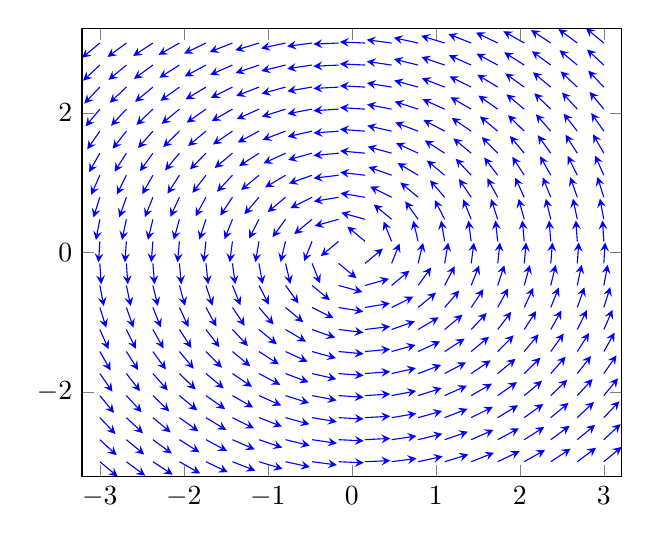
\begin{tikzpicture}
            \def\length{.5*sqrt(x^2+y^2)}
            \begin{axis}[domain=-3:3, view={0}{90}]
                \addplot3[blue, quiver={u={-y/(\length)}, v={x/(\length)}, scale arrows=0.15}, -stealth,samples=20] {0};
            \end{axis}
        \end{tikzpicture}
        \caption{
            \(
            \begin{bmatrix}
                \frac{-y}{\sqrt{x^2+y^2}} & \frac{x}{\sqrt{x^2+y^2}}
            \end{bmatrix}
            \)
        }\label{subfig:vecfield1}
    \end{subfigure}
    \vskip\baselineskip
    \begin{subfigure}[b]{\subfigwidth}
        \centering
        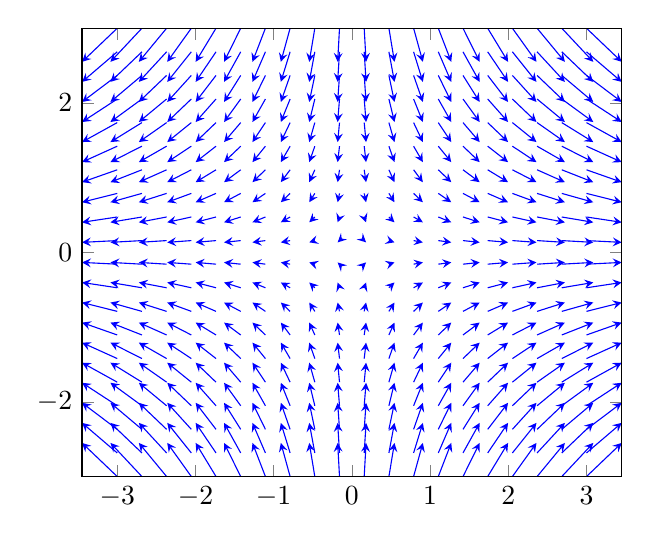
\begin{tikzpicture}
            \begin{axis}[domain=-3:3, view={0}{90}]
                \addplot3[blue, quiver={u={x}, v={-y}, scale arrows=0.15}, -stealth,samples=20] {0};
            \end{axis}
        \end{tikzpicture}
        \caption{
            \(
            \begin{bmatrix}
                x & y
            \end{bmatrix}
            \)
        }\label{subfig:vecfield2}
    \end{subfigure}
    \caption{Vector fields.}\label{fig:vectorfields}
\end{figure}
%</vecfields>

%<*coordinatechart>
\begin{figure*}
    \newcommand*{\scale}{1.5}
    \centering
    \begin{tikzpicture}[thick,scale=\scale, every node/.style={scale=\scale}]
        \path[->] (0.8, 0) edge [bend right] node[left, xshift=-2mm] {$\phi_i$} (-1, -2.9);
        \draw[white,fill=white] (0.06,-0.57) circle (.15cm);
        \path[->] (-0.7, -3.05) edge [bend right] node [right, yshift=-3mm] {$\phi^{-1}$} (1.093, -0.11);
        \draw[white, fill=white] (0.95,-1.2) circle (.15cm);

        % Functions j
        \path[->] (5.8, -2.8) edge [bend left] node[midway, xshift=-5mm, yshift=-3mm] {$\psi^{-1}$} (3.8, -0.35);
        \draw[white, fill=white] (4,-1.1) circle (.15cm);
        \path[->] (4.2, 0) edge [bend left] node[right, xshift=2mm] {$\psi$} (6.2, -2.8);
        \draw[white, fill=white] (4.54,-0.12) circle (.15cm);

        % Manifold
        \draw[smooth cycle, tension=0.4, fill=white, pattern color=brown, pattern=north west lines, opacity=0.7] plot coordinates{(2,2) (-0.5,0) (3,-2) (5,1)} node at (3,2.3) {$M$};

        % Help lines
        %\draw[help lines] (-3,-6) grid (8,6);

        % Subsets
        \draw[smooth cycle, pattern color=orange, pattern=crosshatch dots]
        plot coordinates {(1,0) (1.5, 1.2) (2.5,1.3) (2.6, 0.4)}
        node [label={[label distance=-0.3cm, xshift=-2cm, fill=white]:$U$}] {};
        \draw[smooth cycle, pattern color=blue, pattern=crosshatch dots]
        plot coordinates {(4, 0) (3.7, 0.8) (3.0, 1.2) (2.5, 1.2) (2.2, 0.8) (2.3, 0.5) (2.6, 0.3) (3.5, 0.0)}
        node [label={[label distance=-0.8cm, xshift=.75cm, yshift=1cm, fill=white]:$V$}] {};

        % First Axis
        \draw[thick, ->] (-3,-5) -- (0, -5) node [label=above:$\phi(U)$] {};
        \draw[thick, ->] (-3,-5) -- (-3, -2) node [label=right:$\mathbb{R}^n$] {};

        % Arrow from i to j
        \draw[->] (0, -3.85) -- node[midway, above]{$\psi \circ \phi^{-1}$} (4.5, -3.85);
        \draw[<-] (0,-4.05) -- node[midway, below]{$\phi \circ \psi^{-1}$} (4.5, -4.05);

        % Second Axis
        \draw[thick, ->] (5, -5) -- (8, -5) node [label=above:$\psi(V)$] {};
        \draw[thick, ->] (5, -5) -- (5, -2) node [label=right:$\mathbb{R}^n$] {};

        % Sets in R^m
        \draw[white, pattern color=orange, pattern=crosshatch dots] (-0.67, -3.06) -- +(180:0.8) arc (180:270:0.8);
        \fill[even odd rule, white] [smooth cycle] plot coordinates{(-2, -4.5) (-2, -3.2) (-0.8, -3.2) (-0.8, -4.5)} (-0.67, -3.06) -- +(180:0.8) arc (180:270:0.8);
        \draw[smooth cycle] plot coordinates{(-2, -4.5) (-2, -3.2) (-0.8, -3.2) (-0.8, -4.5)};
        \draw (-1.45, -3.06) arc (180:270:0.8);

        \draw[white, pattern color=blue, pattern=crosshatch dots] (5.7, -3.06) -- +(-90:0.8) arc (-90:0:0.8);
        \fill[even odd rule, white] [smooth cycle] plot coordinates{(7, -4.5) (7, -3.2) (5.8, -3.2) (5.8, -4.5)} (5.7, -3.06) -- +(-90:0.8) arc (-90:0:0.8);
        \draw[smooth cycle] plot coordinates{(7, -4.5) (7, -3.2) (5.8, -3.2) (5.8, -4.5)};
        \draw (5.69, -3.85) arc (-90:0:0.8);
    \end{tikzpicture}
    \caption{Compatible coordinate charts.}\label{fig:compatcoordcharts}
\end{figure*}
%</coordinatechart>

%<*circlatlas>
\begin{figure*}
    \centering
    \includegraphics[width=\textwidth]{figures/chartsoncircle.png}
    \caption{Atlas of charts on the circle.}\label{fig:chartsoncircle}
\end{figure*}
%</circlatlas>
%<*chartsoncirc>
\begin{figure}
    \centering
    \includegraphics[width=\linewidth]{figures/xychartsoncircle.png}
    \caption{Atlas of charts on the circle.}\label{fig:xychartsoncircle}
\end{figure}
%</chartsoncirc>

%<*smoothatapoint>
\begin{figure}
    \centering
    \includegraphics[width=\linewidth]{figures/smoothatapoint.png}
    \caption{Smooth at a point.}\label{fig:smoothatapoint}
\end{figure}
%</smoothatapoint>

%<*smoothf>
\begin{figure}
    \centering
    \includegraphics[width=\textwidth]{figures/smoothF.png}
    \caption{Smooth at a point.}\label{fig:smoothf}
\end{figure}
%</smoothf>

%<*curvevec>
\begin{figure*}
    \centering
    \includegraphics[width=\linewidth]{figures/curvevector.png}
    \caption{Existence of a curve through a point with a given initial vector.}\label{fig:curvevec}
\end{figure*}
%</curvevec>

%<*smoothsec>
\begin{figure}
    \centering
    \includegraphics[width=\linewidth]{figures/smoothsection.png}
    \caption{A section of a vector bundle.}\label{fig:smoothsec}
\end{figure}
%</smoothsec>

%<*tangentbundle>
\begin{figure}
    \centering
    \includegraphics[width=\linewidth]{figures/tangentbundle.png}
    \caption{Tangent bundle to \(S^1\).}\label{fig:tangentbundle}
\end{figure}
%</tangentbundle>

%<*vecfield>
\begin{figure}
    \centering
    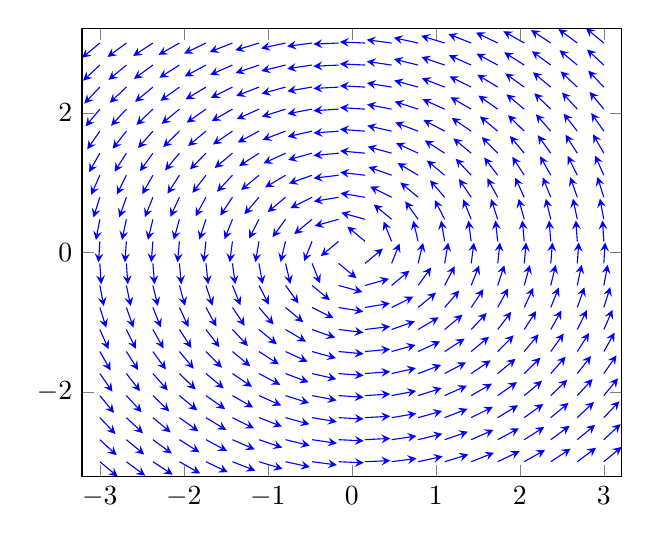
\begin{tikzpicture}
        \def\length{.5*sqrt(x^2+y^2)}
        \begin{axis}[domain=-3:3, view={0}{90}]
            \addplot3[blue, quiver={u={-y/(\length)}, v={x/(\length)}, scale arrows=0.15}, -stealth,samples=20] {0};
        \end{axis}
    \end{tikzpicture}
    \caption{Vector field \(X_{(x,y)} = \frac{1}{\sqrt{x^2+y^2}} \left( -y \pdv{x} + x \pdv{y} \right)\)}\label{fig:vecfield}
\end{figure}
%</vecfield>
\localtableofcontents

Artificial Neural Network (ANN or simply NN) algorithms for SR are all based on a Convolutional Neural Network (CNN) architecture.
%
We first, briefly, review ANNs in general, CNNs in particular, powerful architectures called Deep Neural Networks (DNNs), and a training methodology for networks called Generative Adversarial Networks (GANs).
%
We then proceed to review applications of ANNs to super resolution.
%
\subsection{Basics}
\begin{figure*}[!htbp]
    % MLP
    \centering
    \tikzstyle{inputNode}=[draw,fill=sail,circle,minimum size=10pt,inner sep=2pt]
    \tikzstyle{hiddenNode}=[draw,fill=snowymint,circle,minimum size=10pt,inner sep=2pt]
    \tikzstyle{outputNode}=[draw,fill=plum,circle,minimum size=10pt,inner sep=2pt]
    \tikzstyle{stateTransition}=[-stealth, thick]
    \begin{subfigure}[b]{0.49\textwidth}
        \centering
        \begin{tikzpicture}
            \node[draw,fill=plum, circle,minimum size=25pt,inner sep=0pt] (x) at (0,0) {$\Sigma$ $\sigma$};
            \draw[dashed] (0,-0.43) -- (0,0.43);

            \node[inputNode] (x0) at (-2, 1.5) {$ x_1$};
            \node[inputNode] (x1) at (-2, 0.75) {$ x_2$};
            \node[inputNode] (x2) at (-2, 0) {$ x_3$};
            \node[inputNode] (x3) at (-2, -0.75) {$ x_4$};
            \node[inputNode] (xn) at (-2, -1.95) {$ x_n$};

            \draw[stateTransition] (x0) to[out=0,in=120] node [midway, sloped, above] {$w_1$} (x);
            \draw[stateTransition] (x1) to[out=0,in=150] node [midway, sloped, above] {$w_2$} (x);
            \draw[stateTransition] (x2) to[out=0,in=180] node [midway, sloped, above] {$w_3$} (x);
            \draw[stateTransition] (x3) to[out=0,in=210] node [midway, sloped, above] {$w_4$} (x);
            \draw[stateTransition] (xn) to[out=0,in=240] node [midway, sloped, above] {$w_n$} (x);
            \draw[stateTransition] (x) -- (4,0) node [midway,above] {$z(\mathbf{x}) = \sigma\left(\sum\limits_{i=1}^{n}{w_ix_i} +  b\right)$};
            \node (dots) at (-2, -1.25) {$\vdots$};
        \end{tikzpicture}
        \caption{Single Artificial Neuron function.}\label{fig:singleann}
    \end{subfigure}
    \begin{subfigure}[b]{0.49\textwidth}
        \centering
        \begin{tikzpicture}

            \node[inputNode, thick] (i1) at (6, 0.75) {$x_1$};
            \node[inputNode, thick] (i2) at (6, 0) {$x_2$};
            \node[] (i4) at (6, -0.75) {$\LARGE \vdots$};
            \node[inputNode, thick] (i3) at (6, -1.5) {$x_n$};

            \node[hiddenNode, thick] (h1) at (8, 1.5) {$z_1$};
            \node[hiddenNode, thick] (h2) at (8, 0.75) {$z_2$};
            \node[hiddenNode, thick] (h3) at (8, 0) {$z_3$};
            \node[] (h4) at (8, -0.75) {$\LARGE \vdots$};
            \node[]  at (8, -1.5) {$\LARGE \vdots$};
            \node[hiddenNode, thick] (h5) at (8, -2.25) {$z_m$};

            \node[outputNode, thick] (o2) at (10, 0) {$\Sigma$ $\sigma$};
            \draw[dashed] (10,-0.43) -- (10,0.43);

            \draw[stateTransition] (i1) -- (h1);
            \draw[stateTransition] (i1) -- (h2);
            \draw[stateTransition] (i1) -- (h3);
            \draw[stateTransition] (i1) -- (h5);
            \draw[stateTransition] (i2) -- (h1);
            \draw[stateTransition] (i2) -- (h2);
            \draw[stateTransition] (i2) -- (h3);
            \draw[stateTransition] (i2) -- (h5);
            \draw[stateTransition] (i3) -- (h1);
            \draw[stateTransition] (i3) -- (h2);
            \draw[stateTransition] (i3) -- (h3);
            \draw[stateTransition] (i3) -- (h5);

            \draw[stateTransition] (h1) -- (o2);
            \draw[stateTransition] (h2) -- (o2);
            \draw[stateTransition] (h3) -- (o2);
            \draw[stateTransition] (h5) -- (o2);

            \node[above=of i1, align=center] (l1) {\footnotesize $n$ Neuron \\ \footnotesize Input \\ \footnotesize layer};
            \node[right=1.3em of l1, align=center] (l2) {\footnotesize $m$ Neuron \\ \footnotesize Hidden \\ \footnotesize layer};
            \node[right=2.3em of l2, align=center] (l3) {\footnotesize Output \\ \footnotesize layer};

            \draw[stateTransition] (o2) -- node[midway,above] {$y(\mathbf{x}) = \sigma'\left(\sum\limits_{j=1}^{m}{w'_jz_j} + b'\right)$} (13, 0);
        \end{tikzpicture}
        \caption{Multi-layer ANN.}\label{fig:multiann}
    \end{subfigure}
    \caption{Artificial Neural Network representation.}\label{fig:ann}
\end{figure*}

An ANN is a function specified by composing elementary functions called \newterm{artificial neurons}\anote{ann} (or simply neurons).
%
Neurons consist of a set of inputs \(\mathbf{x} \coloneqq (x_1, x_2, \dots, x_n)\), a set of parameters called weights \(w_i\), and an \newterm{activation function} \(\sigma\), which acts as a thresholding mechanism.
%
For example, the simplest function that qualifies as a neuron is a linear function:
\begin{equation}
    z(\mathbf{x}) = w_1 x_1 + w_2 x_2 = \sum_i w_i x_i
    \label{eqn:simpleann}
\end{equation}
where the activation function is the trivial one the identity.
%
Common non-trivial activation functions are the sigmoid function
\begin{equation}
    \operatorname{sig}(x)={\frac {1}{1+e^{-x}}}={\frac {e^{x}}{e^{x}+1}}
\end{equation}
the hyperbolic tangent function
\begin{equation}
    \tanh x={\frac {\sinh x}{\cosh x}}={\frac {e^{x}-e^{-x}}{e^{x}+e^{-x}}}={\frac {e^{2x}-1}{e^{2x}+1}}
\end{equation}
and the piecewise defined \newterm{rectified linear unit} (\(\operatorname{ReLU}\)):
\begin{align}
    \operatorname{ReLU}(x) & \coloneqq \begin{cases}x&{\text{if }}x>0,\\0&{\text{otherwise}}\end{cases} 
                        %    & = \max(0, x)
\end{align}
Note that eqn.~\eqref{eqn:simpleann} passes through the origin \((0,0,0)\) since it has no constant term; in the parlance of machine learning (ML) the neuron is missing a bias term\anote{bias} \(b\):
\begin{equation}
    z(\mathbf{x}) = \sum_i w_i x_i + b
    \label{eqn:linearregr}
\end{equation}

Neurons can be represented as directed graphs, where a vertex represents an input and edges represent the weights (see figure~\ref{fig:singleann}).
%
ANNs are, then, assemblies of neurons grouped into \newterm{layers} with the layers composed by applying neurons to outputs from immediately preceding layers.
%
For example the ANN specified in figure~\ref{fig:multiann} represents the function
\begin{equation}
    \begin{split}
        y(\mathbf{x}) &= \sigma' \left( \sum_j w'_j z_j(\mathbf{x}) + b' \right) \\
        &=  \sigma' \left( \sum_{j=1}^m w'_j \sigma\left(\sum_{i=1}^n w_i x_i + b_j\right) + b' \right)
    \end{split}
\end{equation}
%
Layers are categorized as either \newterm{hidden layers} or input-output layers: those layers that are not input or output layers are hidden layers.

ANNs seem like a very simple class of functions; for example, Minsky \etal \cite{minsky2017perceptrons} famously proved that single-layer ANNs that don't include a nonlinear activation function can't represent \(\operatorname{XOR}\)\anote{xor}. 
%
On the contrary, strikingly, ANNs that do include a nonlinear activation function satisfy a \newterm{universal approximation theorem} \cite{cybenko1989approximation}:
%
given any continuous function \(f\) (on some bounded interval \(I\)) there exists a sequence of ANNs (with at least one hidden layer and employing a nonlinear activation function) whose limit approximates\anote{uniformconv} \(f\) to arbitrary precision.

A critical component of the universal approximation theorem is finding the correct sequence of ANNs; in the parlance of ML an ANN demands a \newterm{learning rule}.
%
In general, ANN learning rules iterate on the weights \(w_i\) given \(k \gg 1\) \newterm{training} pairs of known \newterm{samples} and \newterm{targets} \(\left\{ \bm{x}_k, t_k \right\}\) of \(f\). 
%
The most common such learning rule is a \newterm{gradient descent} based rule called the Delta rule \cite{widrow1960adaptive}.
%
It is derived from minimizing the \(L_2\) loss with respect to each of the weights using gradient descent:
\begin{equation}
    L(w_1, \dots, w_n) \coloneqq \sum_k \frac{1}{2} (t_k - y(\mathbf{x}_k))^2
    \label{eqn:loss}
\end{equation}
and hence
\begin{equation}
    \pd{L}{w_i} = - \sum_k(t_k-y(\bm{x}_k))\cdot y'\cdot x_{ik}
\end{equation}
where by \(y' \coloneqq \sigma'\) we mean the derivative of the activation function with respect to its argument and by \(x_{ik}\) we mean the \(i\)-th input \(x_i\) of the \(k\)-th training sample \(\bm{x}_k\).
%
Hence, by gradient descent, the weights \(w_i\) should be adjusted in the opposite direction of \(\pd{L}{w_i}\) and we have the weight update rule
\begin{equation}
    \Delta w_i \coloneqq \alpha \cdot \sum_k(t_k-y(\mathbf{x}_k))\cdot \sigma'\cdot x_{ik}
    \label{eqn:batchupdate}
\end{equation}
where \(\alpha\) is a small constant called the \newterm{learning rate} (that controls the rate of convergence of the ANN).

In general, deriving the partial derivatives \(\pd{L}{w_i}\) for a multi-layer, wide (many neurons in each layer) network is compute intensive due to dependencies between weights in adjacent layers.
%
\begin{figure}[!htbp]
    \centering
    \begin{subfigure}[b]{.49\textwidth}
        \centering
        \begin{tikzpicture}[]
            \def\pindist{35pt}
            \def\nodesize{38pt}

            \tikzstyle{every pin edge}=[signal]
            \tikzstyle{annot} = [text width=4em, text centered]

            \node[hiddennode, text width=\nodesize, minimum size=\nodesize,
                pin={[pin edge={latex-}, pin distance=\pindist]above left:$w_1 x_1$},
                pin={[pin edge={latex-}, pin distance=\pindist]below left:$w_2 x_2$},
                pin={[pin edge={-latex}, pin distance=\pindist]right:$y$}
            ] (N1) at (-100pt,0) {$\Sigma\quad \sigma$};
            \draw[dashed] (-100pt,-0.55) -- (-100pt,0.55);
        \end{tikzpicture}
        \caption{Forward Pass.}
    \end{subfigure}
    \vskip\baselineskip
    \begin{subfigure}[b]{.49\textwidth}
        \centering
        \begin{tikzpicture}[]
            \def\pindist{35pt}
            \def\nodesize{38pt}
            \tikzstyle{every pin edge}=[signal]
            \tikzstyle{annot} = [text width=4em, text centered]

            \node[hiddennode, text width=\nodesize, minimum size=\nodesize,
                pin={[pin edge={-latex}, pin distance=\pindist]above left:$\frac{\partial L}{\partial w_1}=\frac{\partial L}{\partial y}\frac{\partial y}{\partial w_1}$},
                pin={[pin edge={-latex}, pin distance=\pindist]below left:$\frac{\partial L}{\partial w_2}=\frac{\partial L}{\partial y}\frac{\partial y}{\partial w_2}$},
                pin={[pin edge={latex-}, pin distance=\pindist]right:$\frac{\partial L}{\partial y}$}
            ] (N2) at (+120pt,0) {$\dif \sigma$};
        \end{tikzpicture}
        \caption{Backwards Pass. Note that \(\pd{L}{y}\) can be reused when computing both \(\pd{L}{w_1}\) and \(\pd{L}{w_2}\).}
    \end{subfigure}
    \caption{Back-propagation computation of derivatives.}\label{fig:backprop}
\end{figure}

Fortunately traversing the derivative-dependency graph in a particular order, a technique called \newterm{back-propagation}\anote{backprop} or simply backprop (see figure~\ref{fig:backprop}), makes this tractable.

Another inefficiency of the Delta rule is that it requires evaluating the ANN on the entire set of samples in order to compute the update \(\Delta w_i\).
%
For large training sets (on the order of millions of samples) this is infeasible due to memory limitations.
%
Stochastic Gradient Descent (SGD) replaces computing the total loss in eqn.~\eqref{eqn:batchupdate} with computing a partial loss called the \newterm{batch loss}:
\begin{equation}
    \Delta w_i^t = w_i^t - w_i^{t-1} \coloneqq \alpha \cdot \sum_j (t_j-y(\mathbf{x}_j))\cdot \sigma'\cdot x_{ij}
    \label{eqn:sgd}
\end{equation}
where the sum on the right-hand side is now over a subset of samples called a \newterm{batch}.
%
This in effect computes the weight update \(\Delta w_i\) incrementally and saves having to hold all training data in memory concurrently.
%
The disadvantage of using SGD is that the batch loss is a noisy estimate of the total loss; in order to assure convergence one typically trains and retrains ANNs on random shufflings of the training data.
%
Each such training episode is called an \newterm{epoch}.
%
% Equation~\eqref{eqn:sgd} is evaluated for each of the \(k\) samples sequentially and therefore saves having to store all training samples in memory.





\subsubsection{Convolutional Neural Networks}




The one-dimensional (1D) discrete convolution \((f*g)\) of 1D discrete functions \(f,g\) is defined
\begin{equation}
    (f*g)[n]\coloneqq \sum _{i} f[i]g[n-i]
    \label{eqn:1dconv}
\end{equation}
The convolution of a function \(f\) with a finite sequence of values \(g\) can be interpreted as filtering \(f\) with the filter \(g\); for example convolving a noisy \(f\) with a Heaviside function smoothes \(f\) (see figure~\ref{fig:convfiltering}).
\begin{figure}[!htbp]
    \centering
    \begin{subfigure}[b]{.49\textwidth}
        \centering
        \includegraphics[width=0.95\textwidth]{figures/neural_networks/unsmoothed.png}
        \caption{Noisy function \(f\) (Gaussian process sample).}\label{fig:convnoisy}
    \end{subfigure}

    \begin{subfigure}[b]{.49\textwidth}
        \centering
        \includegraphics[width=0.95\textwidth]{figures/neural_networks/kernel.png}
        \caption{Heaviside function (low-pass filter \(g\)).}\label{fig:convfilter}
    \end{subfigure}
    \begin{subfigure}[b]{.49\textwidth}
        \centering
        \includegraphics[width=0.95\textwidth]{figures/neural_networks/smoothed.png}
        \caption{Smoothed (low-pass filtered) \(f * g\).}\label{fig:convsmooth}
    \end{subfigure}
    \caption{Convolution as filtering.}\label{fig:convfiltering}
\end{figure}
%
The sequence of values that comprise \(g\) is called the \newterm{kernel} of the \(g\) and the length of the sequence is called the \newterm{bandwidth} of the kernel (or simply width).
%
The two-dimensional (2D) discrete convolution \((f*g)\) of 2D discrete functions \(f,g\) is defined
\begin{equation}
    (f*g)[n, m]\coloneqq \sum _{i}\sum _{j}f[i, j]g[n-i, m-j]
    \label{eqn:2dconv}
\end{equation}
and can be interpreted in exactly the same way as 1D convolutions.
%
For 2D convolutions the kernels are most often square and therefore the kernel dimensions are specified rather than just width (see figure~\ref{fig:2dconv}).
\begin{figure*}
    \centering

    \tikzset{
        inputsquare/.pic={
                \draw[fill=sail] (0,0) rectangle (4,4);
                \draw[black, thick] (0,0) grid (4,4);
                \node at (0.5,0.5) {2};
                \node at (0.5,1.5) {3};
                \node at (0.5,2.5) {0};
                \node at (0.5,3.5) {3};
                \node at (1.5,0.5) {2};
                \node at (1.5,1.5) {1};
                \node at (1.5,2.5) {0};
                \node at (1.5,3.5) {3};
                \node at (2.5,0.5) {3};
                \node at (2.5,1.5) {3};
                \node at (2.5,2.5) {0};
                \node at (2.5,3.5) {2};
                \node at (3.5,0.5) {2};
                \node at (3.5,1.5) {1};
                \node at (3.5,2.5) {1};
                \node at (3.5,3.5) {1};
            },
        pics/filtersquare/.style args={#1/#2/#3/#4}{
                code = {
                        \draw[fill=snowymint] (#1,#2) rectangle (#3,#4);
                        \draw[black, thick] (#1,#2) grid (#3,#4);
                        \node at (#1+0.5,#2+0.5) {0};
                        \node at (#1+0.5,#2+1.5) {2};
                        \node at (#1+0.5,#2+2.5) {0};
                        \node at (#1+1.5,#2+0.5) {0};
                        \node at (#1+1.5,#2+1.5) {2};
                        \node at (#1+1.5,#2+2.5) {0};
                        \node at (#1+2.5,#2+0.5) {1};
                        \node at (#1+2.5,#2+1.5) {0};
                        \node at (#1+2.5,#2+2.5) {2};
                    }},
        pics/outputsquare/.style args={#1/#2/#3/#4}{
                code = {
                        \draw[fill=plum] (0,0) rectangle (2,2);
                        \draw[black, thick] (0,0) grid (2,2);
                        \node at (0.5,0.5) {#3};
                        \node at (0.5,1.5) {#1};
                        \node at (1.5,0.5) {#4};
                        \node at (1.5,1.5) {#2};
                    }}
    }
    \newcommand*{\figwidth}{.25}
    \newcommand*{\figscale}{1}
    \begin{subfigure}[b]{\textwidth}
        \centering
        \begin{tikzpicture}[scale=1,every node/.style={minimum size=1cm},on grid]
            \node (node) at (-0.5,2) {$f = $};
            \pic {inputsquare};
            \begin{scope}[xshift=5cm, yshift=0.5cm]
                \node (node) at (-0.5,1.5) {$g = $};
                \pic {filtersquare=0/0/3/3};
            \end{scope}
            \begin{scope}[xshift=9.5cm, yshift=1cm]
                \node (node) at (-0.75,1) {$f * g = $};
                \pic {outputsquare=7/3/11/12};
            \end{scope}
        \end{tikzpicture}
        \caption{Input \(f\), 2D \(3 \times 3\) convolution kernel \(g\), and output \(f * g\).}
    \end{subfigure}
    \vskip\baselineskip
    \begin{subfigure}[b]{\textwidth}
        \centering
        \begin{tikzpicture}[scale=\figscale,every node/.style={minimum size=1cm},on grid]
            \begin{scope}[every node/.append style={yslant=0.5,xslant=-0.7},
                    yslant=0.5,xslant=-0.7]

                \pic {inputsquare};
                \coordinate (BL) at (0,1);
                \coordinate (BR) at (3,1);
                \coordinate (TL) at (0,4);
                \coordinate (TR) at (3,4);
            \end{scope}
            \begin{scope}[
                    xshift=-.4,
                    yshift=.4cm,
                    every node/.append style={yslant=0.5,xslant=-0.7,opacity=.4},
                    yslant=0.5,xslant=-0.7]
                \pic{filtersquare=0/1/3/4};

                \coordinate (EBL) at (0,1);
                \coordinate (EBR) at (3,1);
                \coordinate (ETL) at (0,4);
                \coordinate (ETR) at (3,4);

            \end{scope}
            \begin{scope}[xshift=-5, yshift=5cm,
                    every node/.append style={yslant=0.5,xslant=-0.7},
                    yslant=0.5,xslant=-0.7]

                \draw (EBL) -- (0,1) (EBR) -- (1,1)
                (ETL) -- (0,2)    (ETR) -- (1,2);

                \draw (EBL) -- (BL) (EBR) -- (BR)
                (ETL) -- (TL)     (ETR) -- (TR);

                \pic{outputsquare=7/0/0/0};
            \draw[fill=black, opacity=0.3] (0,1) rectangle (1,2);

            \end{scope}
        \end{tikzpicture}
        \begin{tikzpicture}[scale=\figscale,every node/.style={minimum size=1cm},on grid]
            \begin{scope}[every node/.append style={yslant=0.5,xslant=-0.7},
                    yslant=0.5,xslant=-0.7]
                \pic{inputsquare};
                \coordinate (BL) at (1,1);
                \coordinate (BR) at (4,1);
                \coordinate (TL) at (1,4);
                \coordinate (TR) at (4,4);
            \end{scope}
            \begin{scope}[
                    xshift=-.4,
                    yshift=.4cm,
                    every node/.append style={yslant=0.5,xslant=-0.7,opacity=.4},
                    yslant=0.5,xslant=-0.7]

                \pic{filtersquare=1/1/4/4};

                \coordinate (EBL) at (1,1);
                \coordinate (EBR) at (4,1);
                \coordinate (ETL) at (1,4);
                \coordinate (ETR) at (4,4);
            \end{scope}
            \begin{scope}[xshift=-5, yshift=5cm,
                    every node/.append style={yslant=0.5,xslant=-0.7},
                    yslant=0.5,xslant=-0.7]
                \draw (EBL) -- (1,1) (EBR) -- (2,1)
                (ETL) -- (1,2)    (ETR) -- (2,2);
                \draw (EBL) -- (BL) (EBR) -- (BR)
                (ETL) -- (TL)    (ETR) -- (TR);

                \pic{outputsquare=7/3/0/0};
                \draw[fill=black, opacity=0.3] (1,1) rectangle (2,2);

            \end{scope}
        \end{tikzpicture}

        \begin{tikzpicture}[scale=\figscale,every node/.style={minimum size=1cm},on grid]
            \begin{scope}[every node/.append style={yslant=0.5,xslant=-0.7},
                    yslant=0.5,xslant=-0.7]
                \pic{inputsquare};
                \coordinate (BL) at (0,0);
                \coordinate (BR) at (3,0);
                \coordinate (TL) at (0,3);
                \coordinate (TR) at (3,3);
            \end{scope}
            \begin{scope}[
                    xshift=-.4,
                    yshift=.4cm,
                    every node/.append style={yslant=0.5,xslant=-0.7,opacity=.4},
                    yslant=0.5,xslant=-0.7]
                \pic{filtersquare=0/0/3/3};

                \coordinate (EBL) at (0,0);
                \coordinate (EBR) at (3,0);
                \coordinate (ETL) at (0,3);
                \coordinate (ETR) at (3,3);
            \end{scope}
            \begin{scope}[xshift=-5, yshift=5cm,
                    every node/.append style={yslant=0.5,xslant=-0.7},
                    yslant=0.5,xslant=-0.7]
                \draw (EBL) -- (0,0) (EBR) -- (1,0)
                (ETL) -- (0,1)    (ETR) -- (1,1);
                \draw (EBL) -- (BL) (EBR) -- (BR)
                (ETL) -- (TL)    (ETR) -- (TR);

                \pic{outputsquare=7/3/11/0};
                \draw[fill=black, opacity=0.3] (0,0) rectangle
                (1,1);

            \end{scope}
        \end{tikzpicture}
        \begin{tikzpicture}[scale=\figscale,every node/.style={minimum size=1cm},on grid]
            \begin{scope}[every node/.append style={yslant=0.5,xslant=-0.7},
                    yslant=0.5,xslant=-0.7]
                \pic{inputsquare};

                \coordinate (BL) at (1,0);
                \coordinate (BR) at (4,0);
                \coordinate (TL) at (1,3);
                \coordinate (TR) at (4,3);
            \end{scope}
            \begin{scope}[
                    xshift=-.4,
                    yshift=.4cm,
                    every node/.append style={yslant=0.5,xslant=-0.7,opacity=.4},
                    yslant=0.5,xslant=-0.7]
                \pic{filtersquare=1/0/4/3};
                \coordinate (EBL) at (1,0);
                \coordinate (EBR) at (4,0);
                \coordinate (ETL) at (1,3);
                \coordinate (ETR) at (4,3);
            \end{scope}
            \begin{scope}[xshift=-5, yshift=5cm,
                    every node/.append style={yslant=0.5,xslant=-0.7},
                    yslant=0.5,xslant=-0.7]
                \draw (EBL) -- (1,0) (EBR) -- (2,0)
                (ETL) -- (1,1)    (ETR) -- (2,1);
                \draw (EBL) -- (BL) (EBR) -- (BR)
                (ETL) -- (TL)    (ETR) -- (TR);
                \pic{outputsquare=7/3/11/12};
                \draw[fill=black, opacity=0.3] (1,0) rectangle (2,1);

            \end{scope}
        \end{tikzpicture}
        \caption{Evaluation of convolution.}\label{fig:2dconviter}
    \end{subfigure}
    \caption{2D convolution.}\label{fig:2dconv}
\end{figure*}

Notice that eqns.~\eqref{eqn:1dconv} and~\eqref{eqn:2dconv} are completely linear in their inputs \(f[i]\) (\(f[i,j]\)) with weights \(w_i = g[n-i]\) (\(w_{ij} = g[n-i, m-j]\)) and hence naturally constitute a neuron (layer of neurons); a \newterm{convolution layer} in a multi-layer ANN is either eqn.~\eqref{eqn:1dconv} or eqn.~\eqref{eqn:2dconv} with kernel values being iteratively updated by the learning rule.
%
Hence, a CNN is an ANN with one or more convolution layers; CNNs consisting of 2D convolutions are particularly effective for tasks that operate on images (since image patches have more structure than image slices).

In practice multiple filters are applied to the same input and then stacked to produce a higher-dimensional output (see figure~\ref{fig:multconvs}), each dimension of which is called a \newterm{feature map}.
\begin{figure}
    \centering
    \begin{tikzpicture}[scale=.35,every node/.style={minimum size=1cm}, on grid]
        \begin{scope}[]
            \node (node) at (-1.5,2) {$f = $};
            \draw[draw=base03,fill=blue,thick]
            (0,0) grid (4,4) rectangle (0,0);
        \end{scope}

        \foreach \x [count=\i] in {-7,0,7} {%
                \begin{scope}[xshift=\x cm,yshift=8cm]
                    \begin{scope}[xshift=0.5cm,yshift=0.5cm]
                        \node (node) at (-1.5,1.5) {$g_\i = $};
                        \draw[step=10mm, base03, thick] (0,0) grid (3,3);
                        \draw[fill=base02, opacity=0.4]
                        (0,0) grid (3,3) rectangle (0,0);
                    \end{scope}
                \end{scope}
                \begin{scope}[xshift=\x cm,yshift=16cm]
                    \begin{scope}[xshift=1cm]
                        \node (node) at (-2.5,1) {$f * g_\i = $};
                        \draw[draw=base03,fill=cyan,thick]
                        (0,0) grid (2,2) rectangle (0,0);
                    \end{scope}
                \end{scope}
            }

        \begin{scope}[xshift=1cm,yshift=24cm]
            \node (node) at (-2,1) {$f' = $};
            \foreach \s in {-0.5,0, 0.5} {%
                    \begin{scope}[xshift=\s cm,yshift=\s cm]
                        \draw[draw=base03,fill=cyan,thick]
                        (0,0) grid (2,2) rectangle (0,0);
                    \end{scope}
                }
        \end{scope}
        \draw[thick] (-0.5,3.5)   -- (-5,8);
        \draw[thick] (2,4.5)      -- (2,8) ;
        \draw[thick] (4.5,3.5)    -- (9,8) ;

        \draw[thick] (-5,12) -- (-5,15.5);
        \draw[thick] (2,12) -- (2,15.5)  ;
        \draw[thick] (9,12) -- (9,15.5)  ;

        \draw[thick] (-5,18.5) --(-0.125,23.5);
        \draw[thick] (2,18.5) -- (2,23)   ;
        \draw[thick] (9,18.5) -- (4.125,23.5) ;
    \end{tikzpicture}
    \caption{A convolution layer consisting of three distinct \(3\times 3\) filters.}\label{fig:multconvs}
\end{figure}
%
Depending on whether the CNN is being employed to solve a generative task or a classification task the activation function might be either a \(\operatorname{ReLU}\) (applied element-wise to the output of the convolution layer) or a \newterm{max-pooling} filter:
\begin{multline}
    \operatorname{max-pool}(f,g)[n, m]\coloneqq\\ \max_{i,j}\left[ f[i, j]g[n-i, m-j] \right]
    \label{eqn:2dpool}
\end{multline}
There are many other convolution operators (e.g., strided, dilated, transposed) that are beyond the scope of this survey \cite{dumoulin2016guide}.





\subsubsection{Deep Neural Networks}\label{subsubsec:dnns}





%
Deep Neural Networks (DNNs) are ANNs that have multiple layers and many neurons in each layer.
%
Intuitively the advantage of deep networks (over shallow networks) is they learn\anote{learn} hierarchies of concepts (called \newterm{features}); for example in facial recognition tasks, layers proximal to the input layer learn to recognize elementary features such as edges, layers distal to the input layer learn abstractions of elementary features, such as arrangements of edges that comprise eyes or noses, and layers even more distal to the input layer learn entire faces.

Training DNNs presents many challenges; due to their depth they suffer from issues such as \newterm{vanishing gradients} and \newterm{overfitting}.
%
Vanishing gradients is an all but complete cessation of substantive updates to weights; consider the partial derivative of the activation function \(\sigma'\) in eqn.~\eqref{eqn:batchupdate}.
%
Notice that if \(\abs{\sigma'} \ll 1\) then \(\Delta w_i\) will be very small.
%
This occurs for a single neuron when the input \newterm{saturates} the activation function; for example for \(\operatorname{sig}\) this happens when \(\abs{x} > 5\) because the gradient \(\sigma'\) is very small (see figure~\ref{fig:activs}).
\begin{figure}[!htbp]
    \centering
    \includegraphics[width=\linewidth]{figures/neural_networks/activation_grads.png}
    \caption[]{Sigmoid activation gradients. Note that for \(\abs{x} > 5\) the gradient is almost 0.}\label{fig:activs}
\end{figure}
%
For multi-layer ANNs, such as DNNs, even if no single neuron saturates the activation function,
due to the chain rule, weight updates for layers near the input are proportional to very many factors that are less than one (whose product therefore is near 0).
%
Overfitting, on the other hand, can be interpreted as memorization of the training samples; since the minimization problem (eqn.~\eqref{eqn:loss}) that leads to the Delta rule only measures \(\abs{t_k - y(\mathbf{x}_k)}\), DNNs can simply encode responses to many (or most) of the training samples in their weights (in order to effectively minimize). 
%
This is possible due to DNNs having so many degrees of freedom\anote{largeparams}.

\begin{figure}
    \centering
    \begin{subfigure}[c]{0.49\textwidth}
        \centering
        \includegraphics[width=\textwidth, trim=145 50 145 0, clip]{figures/neural_networks/batch_norm.png}
        \caption[]{Batch normalization's effect, for a single neuron, on inputs to a Sigmoid activation function.}\label{eqn:batchnorm1}
    \end{subfigure}

    \begin{subfigure}[b]{0.49\textwidth}
        \centering
        \begin{tikzpicture}[
            start chain=going below, node distance=12pt,
            point/.append style={on chain, join=by {signal}},
            layer/.append style={on chain, join=by {signal}},
        ]
        \node[point] {Input};
        \node[point] {$\LARGE \vdots$};
        \node[conv] {Conv};
        \node[bn] {BatchNorm};
        \node[activation] {Sigmoid};
        \node[point] {$\LARGE \vdots$};
        \node[point] {Output};
    \end{tikzpicture}
    \caption[]{Batch normalization as a layer in a DNN.}\label{eqn:batchnorm2}
    \end{subfigure}
    \caption[]{Batch normalization.}\label{eqn:batchnorm}
\end{figure}
\input{figures/neural_networks/dropout.tex}
Overfitting and vanishing gradients are only two of the challenges in training sophisticated ANNs.
%
Fortunately there exist a set of practices, called Deep Learning, that make training DNNs feasible.
%
For example, to combat vanishing gradient, Batch Normalization \cite{ioffe2015batch} is used to normalize outputs from linear layers prior to activation (see figure~\ref{fig:batchnorm}).
%
This centering and scaling of the data ensures that no single neuron will saturate its activation function.
%
It operates on a batch by batch basis, \((0,1)-\)Normal normalizing inputs to each layer's activation function:
\begin{align}
    \bm{\mu} _{B}        & \coloneqq {\frac {1}{m}}\sum _{j=1}^{m}\bm{x}_{j}                                             \\
    \bm{\sigma} _{B}^{2} & \coloneqq{\frac {1}{m}}\sum _{j=1}^{m}(\bm{x}_{j}-\bm{\mu}_{B})^{2}                           \\
    {\hat {\bm{x}}}      & \coloneqq {\frac {\bm{x}-\bm{\mu}_{B}}{\sqrt {\bm{\sigma}_{B}^{2}}}} \label{eqn:bathcnormdiv}
\end{align}
where \(m\) is the batch size and the operations in eqn.~\eqref{eqn:bathcnormdiv} are understood to be broadcast (i.e., \(\sqrt {\bm{\sigma} _{B}^{2}}\) is an element-wise root and elements of \(\sqrt {\bm{\sigma} _{B}^{2}}\) divide corresponding elements of \(\bm{x}-\bm{\mu}_{B}\)).
%
In fact Batch normalization actually has two parameters \(\gamma, \beta\) that it learns (using backprop) from the data: the output \(\bm{y}\) after batch normalization is actually defined
\begin{equation}
    \bm{y} \coloneqq \gamma \bm{\hat{x}} + \beta 
\end{equation}
The intuitive reason for learning \(\beta, \gamma\) instead of just fixing them to be \(0,1\) is that \((0,1)\)-Normal normalization isn't necessarily correct in all cases (so why not learn the \((\beta,\gamma)\)-Normal normalization as informed by training data).
%
\begin{figure*}
	\tikzset{
		%Define standard arrow tip
		>=stealth',
		%Define style for boxes
		punkt/.style={
				rectangle,
				rounded corners,
				draw=black, very thick,
				text width=6.5em,
				minimum height=2em,
				text centered
			},
	}
	\begin{adjustbox}{width=\textwidth}
		\begin{tikzpicture}

			\node[] (z) {$\bm{z} \sim \operatorname{N}(0,I)$};
			\node[punkt, fill=sail, right=2em of z] (gen) {Generator};
			\node[below=of gen, inner sep=0pt] (pt7) {};
			\node[above=of gen] (x) {Real image \(\bm{x}\)};
			\node[punkt, fill=plum, right=5em of gen, yshift=2.5em] (discr) {Discriminator};
			\node[above=of discr, inner sep=0pt] (pt8) {};
			\node[punkt, fill=snowymint, right=of discr] (loss) {Loss};
			\node[right=of loss, inner sep=0pt] (pt4) {};
			\node[above=3.85em of pt4, inner sep=0pt] (pt5) {};
			\node[below=6.2em of pt4, inner sep=0pt] (pt6) {};

			\node[right=3em of x, circle, fill, inner sep=0.15em] (pt1) {};
			\node[right=2.5em of gen, circle, fill, inner sep=0.15em] (pt2) {};
			\draw[dashed, thick] (pt1) edge[bend right] (pt2);
			\node[circle, draw, thick, fill=white, inner sep=0.15em] at ([xshift=-0.6em, yshift=3em]pt2.north) (pt3) {};

			\draw[-stealth, thick] (z) -- (gen);
			\draw[-stealth, thick] (pt3) -- (discr.west);
			\draw[-stealth, thick] (discr) -- (loss);
			\draw[-stealth, thick] (gen) -- (pt2);
			\draw[-stealth, thick] (x) -- (pt1);

			\draw[dashed, thick, -stealth] (loss) -- (pt4) -- (pt5) -- node[above] {\(\mathbb{E} [\log D(\bm{x})] + \\ \mathbb{E} [\log(1 - D(G(\bm{z})))]\)} (pt8) -- (discr.north);
			\draw[dashed, thick, -stealth] (loss) -- (pt4) -- (pt6) -- node[above] {\(\mathbb{E} [\log(1 - D(G(\bm{z})))]\)} (pt7) -- (gen.south);


		\end{tikzpicture}
	\end{adjustbox}
	\caption{Schematic diagram for Generative Adversarial Network}\label{fig:gan}

\end{figure*}

\begin{figure}
    \centering

        \begin{tikzpicture}[start chain=going below, node distance=12pt,
            point/.append style={on chain, join=by {signal}},
            layer/.append style={on chain, join=by {signal}},
            branch/.append style={on chain, join=by {signal, -}},
            ]
            \def\branchy{20pt}

            \node[activation] {Layer 1};
            \node[branch] (input) {};
            \node[bn, xshift=\layerwidth/2+16pt, yshift=-\branchy] {Layer 2};
            \node[conv] {Layer 3};
            \node[layer, xshift=-\layerwidth/2-16pt, yshift=-\branchy] (add) {Layer 4};
            \node[point] {Output};
            \draw[signal] (input) -- (add);
        \end{tikzpicture}
    \caption{Skip connection connecting non-adjacent layers.}\label{fig:skipconnection}
\end{figure}
Another solution to the vanishing gradients problem is using \newterm{skip connections}: outputs from a layer can be made to skip adjacent layers early on in training (see figure~\ref{fig:skipconnections}).
%
This has the effect that substantive gradients can be propagated farther back into the network during the initial part of training when weights should be changing the most (since they're ostensibly far from a minimum).

Overfitting in some sense is a problem opposite of vanishing gradients; while vanishing gradients prevent the DNN from learning, overfitting means the DNN is learning too easily.
%
Naturally then, overfitting is mitigated by using regularization; methods such as \(L_2\) regularization and \newterm{dropout} have been shown to be effective against overfitting \cite{bengio2013}.
%
\(L_2\) regularization incorporates a squared weight term \(\frac{\lambda}{2}\sum_{i=1}^n w_i^2\) into eqn.~\eqref{eqn:loss}, which translates into a \newterm{weight decay} term \(\lambda w_i^{t-1}\) in the Delta rule (eqn.~\eqref{eqn:sgd}):
\begin{equation}
    \Delta w_i^t = \alpha \cdot \sum_j (t_j-y(\mathbf{x}_j))\cdot \sigma'\cdot x_{ij} + \lambda w_i^{t-1}
    \label{eqn:weightdecaydelta}
\end{equation}
On the other hand dropout enforces regularization by selectively disabling neurons in the network (see figure~\ref{fig:dropout}); on each forward pass through the network a neuron is either passed input or not according to some probability \(p\) (usually \(p = 0.5\)).
%
The intuition being that not every neuron will have an opportunity to learn from every sample thereby limiting the capacity of the ANN to memorize patterns unique to the training samples.

There are many other best-practices techniques for training DNNs that are beyond the scope of this brief review; an accessible survey is Montavon \etal \cite{montavon2012neural}.




\subsubsection{Generative Adversarial Networks}\label{subsubsec:gan}




A Generative Adversarial Network \cite{goodfellow2014generative} is a training regimen for networks that perform \newterm{generative tasks}.
%
A generative task is one which calls for generating samples from a probability distribution represented by the training data.
%
For example one might have many images of people and one might wish to generate new samples (see figure~\ref{fig:stylegan}) from the probability distribution of such images (i.e., new images of people).
\begin{figure}[!htbp]
    \centering
    \begin{adjustbox}{width=\linewidth}
        \centering
        \includegraphics[]{figures/neural_networks/stylegan.jpg}
    \end{adjustbox}
    \caption{Uncurated set of images \textbf{generated} (i.e., none of the people depicted are real) using StyleGAN with the FFHQ dataset \cite{karras2018stylebased}.}\label{fig:stylegan}
\end{figure}
%
Super-resolution can be cast as a generative task: knowing the condtional distribution of high-frequency components in an image, one could recover said high-frequency components by drawing from that distribution.
%
In general, this is a highly non-trivial problem due to the dimensionality of the sample space.

GANs solve this problem by pitting a \newterm{generator} \(G\), that learns to transform samples from a readily available high-dimensional surrogate distribution (Normal or Uniform), against a \newterm{discriminator} \(D\).
The generator takes as input samples \(\bm{z}\) from the surrogate distribution \(p_{z}\) and outputs putative samples \(G(\bm{z})\) from the real distribution \(p_r\).
%
The discriminator alternates between considering true samples \(\bm{x}\) from the real distribution and considering counterfeit samples \(G(\bm{z})\) produced by the generator; it therefore assesses the quality of \(G\)'s output with respect to its own understanding of the real distribution.
%
To that end Goodfellow \etal \cite{goodfellow2014generative} propose a training framework that involves \(D\) and \(G \) playing a \newterm{mini-max game}\anote{minimax}:
\begin{equation}
    \min_G \max_D L(D, G)
\end{equation}
where
\begin{equation}
    L(D, G) \coloneqq \mathbb{E}_{\bm{x} \sim p_{r}} [\log D(\bm{x})] + \mathbb{E}_{\bm{z} \sim p_{z} } [\log(1 - D(G(\bm{z})))]
    \label{eqn:ganloss}
\end{equation}
Since the discriminator seeks to maximize \(L(D, G)\), the term \(\mathbb{E}_{\bm{x} \sim p_{r}} [\log D(\bm{x})]\) ensures that it is able to correctly identify (i.e., score high) true samples.
%
Simultaneously the term \(\mathbb{E}_{\bm{z} \sim p_{z} } [\log(1 - D(G(\bm{z})))] \) ensures that it is able to correctly identify (i.e., score low) counterfeit samples produced by \(G\).
%
Conversely, \(\mathbb{E}_{\bm{z} \sim p_{z} } [\log(1 - D(G(\bm{z})))]\) (the first term in eqn.~\eqref{eqn:ganloss}) does not play a role when optimizing \(G\)) and so \(G\) is encouraged to improve its ability to fool the discriminator (i.e., produce plausible samples from the real distribution).
%
Goodfellow \etal prove that for the generator this loss criterion is equivalent to minimizing the Jensen–Shannon divergence\anote{kldiv} between the distribution that it models and the true distribution of the data.
\subsection{Deep Neural Networks for SISR}
Deep neural network architectures for single-image super-resolution abide a four tiered hierarchy (according to complexity) which roughly parallels the chronological order of the innovations that have contributed to the current state of the art:
\begin{mdframed}
    \begin{itemize}
        \item \textbf{Pre-defined up-sampling}: networks that expect the image to already have been up-sampled (e.g., using bicubic interpolation). These networks chiefly restore high-frequency features that are omitted by the classical up-sampling technique.
        \item \textbf{Single up-sampling}: networks that perform the up-sampling themselves (in addition to performing restoration).
        \item \textbf{Progressive up-sampling}: networks that up-sample in phases, performing restoration at every phase.
        \item \textbf{Iterative up-sampling}: networks that up-sample and then assess the goodness of the result by down-sampling to original low-resolution (see section~\ref{subsubsec:iterback} for the classical analogue).
    \end{itemize}
\end{mdframed}



\subsubsection{SRCNN and Very Deep SR}\label{subsubsec:vdsr}




The first successful foray of Deep Learning into SISR was the 2-layer Super-Resolution CNN (SRCNN) model \cite{Dong_2016}.
%
SRCNN is a CNN composed of two convolution layers, with the first layer consisting of 64 filters (per color channel), the second layer consisting of 32 filters, and both layers employing \(\operatorname{ReLU}\) activations.
%
Dong \etal argue that their CNN architecture is equivalent to sparse coding SR (see figure~\ref{fig:srcnn}).
\begin{figure}[!htbp]
    \centering
    \newcommand*{\subfigwidth}{0.49\textwidth}
    \begin{subfigure}[b]{\subfigwidth}
        \includegraphics[width=\linewidth,keepaspectratio]{figures/neural_networks/sparse_coding.png}
        \caption{Sparse coding SR pipeline (see section~\ref{subsubsec:sparsecoding}).}\label{subfig:srcnnsparse}
    \end{subfigure}
    \vskip\baselineskip
    \begin{subfigure}[b]{\subfigwidth}
        \includegraphics[width=\linewidth,keepaspectratio]{figures/neural_networks/srcnn.png}
        \caption{SRCNN pipeline.}\label{subfig:srcnn}
    \end{subfigure}
    \caption{Sparse coding SR and SRCNN comparison \cite{Dong_2016}. Note both pipelines operate on bicubic up-sampled images.}\label{fig:srcnn}
\end{figure}
%
This is a common theme in the literature --- ANN architectures learning transformations equivalent to classical techniques --- owing to the universal approximation theorem.

Clearly, at least by modern standards, 2 layers isn't very deep; Dong \etal do experiment with an additional convolution layer but report difficulties maintaining reasonable convergence rates due to vanishing gradients.
%
Kim \etal \cite{Kim_2016} improve on SRCNN with Very Deep SRCNN (VDSR) by increasing the convolution layer count to a sum total of 20.
%
In order to overcome the training challenges faced by Dong \etal they use skip connections (see section~\ref{subsubsec:dnns}).
%
They also use learning rate \newterm{annealing}\anote{annealing} and implement gradient clipping to prevent \newterm{exploding gradients}\anote{gradclip}.
%
They further argue that an SR network need only learn \newterm{residuals} \(\bm{r} \coloneqq \bm{t} - \bm{x}\).
%
In this context, residuals have the significance of being the high-frequency components of an image, since the bicubic up-sampled input \(\bm{x}\) can be interpreted as a low-pass filtered version of the high-resolution image.
%
Hence, their loss function measures the error between the HR image target and the output of the network \(\bm{y}\) plus the input:
\begin{equation}
    L(\bm{t}, \bm{x}) \coloneqq \abs{\bm{t} - (\bm{x} + \bm{y})}^2
\end{equation}
where in the case that \(\bm{y}\) perfectly approximates \(\bm{r}\) the loss would be 0.




\subsubsection{Super-Resolution GAN}\label{subsubsec:srgan}




Single up-sampling networks forgo bicubic pre-processing and learn the up-sampling transformation as a component of the network.
%
The most interesting network in this class of networks is the Super-resolution Residual Network (SRResNet) along with its GAN trained counterpart SRGAN \cite{Ledig_2017}.
%
SRResNet takes as input LR images and similar to VDSR passes them through 16 individual ResBlocks (see figure~\ref{fig:resblock}) for feature extraction.
%
Where SRResNet differs from VDSR is the in-network up-sampling that it performs using \newterm{sub-pixel convolutions}.
%
Sub-pixel convolutions are a way to learn up-sampling as a component of the ANN.
%
They up-sample in two phases: first \(r^2\) filters are convolved with the input, where \(r\) is the up-sampling factor (e.g., 4 filters for 2x up-sampling), then a \newterm{pixel shuffle} operation reorders the elements of the feature maps into an \(r\)-times higher resolution grid (see figure~\ref{subfig:pixelshuffle}).
\begin{figure}[!htbp]
    \centering
    \newcommand*{\subfigwidth}{.49\textwidth}
    \begin{subfigure}[b]{\subfigwidth}
        \centering
        \includegraphics[width=\textwidth]{figures/neural_networks/subpixelconv1.png}
        \caption{Sub-pixel convolution as dilation then filtering.}\label{subfig:subpixdilate}
    \end{subfigure}
    \vskip\baselineskip
    \begin{subfigure}[b]{\subfigwidth}
        \centering
        \includegraphics[width=\textwidth]{figures/neural_networks/subpixelconv2.png}
        \caption{Sub-pixel convolution as filtering then pixel-shuffling.}\label{subfig:pixelshuffle}
    \end{subfigure}
    \caption{Sub-pixel convolution.}\label{fig:subpixelconv}
\end{figure}
%
This operation is called a sub-pixel convolution because it can be interpreted as first dilating the LR image and then convolving with a filter to get a feature map with sub-pixel (relative to the original LR image) responses (see figure~\ref{subfig:subpixdilate}).

Ledig \etal pre-train SRResNet using mean-squared-error (MSE) loss and then further train using the GAN framework (see section~\ref{subsubsec:gan}).
%
In addition to using the conventional GAN loss they add a term called \newterm{perceptual loss}:
\begin{equation}
    \ell_{feat}^{\phi, j} \left( \hat{\bm{y}}, \bm{y}_c\right) \coloneqq \frac{1}{H_j W_j} \abs{\phi_j\left({\hat{\bm{y}}}\right) - \phi_j \left(\bm{y}_c\right)}^2
\end{equation}
where \(\phi_j\) is the \(j\)-th layer activation of the VGG network \cite{simonyan2014very} pretrained on a large data set, \(\hat{\bm{y}}\) is the output of SRResNet, and \(\bm{y}_c\) is the target HR image (see figure~\ref{fig:perceptualloss}), and \(H_j, W_j\) are the dimensions of the \(j\)-th layer activation of VGG.
\begin{figure}[!htbp]
    \centering
    \begin{adjustbox}{width=\linewidth}
        \centering
        \includegraphics[]{figures/neural_networks/perceptual_loss.png}
    \end{adjustbox}
    \caption{Perceptual loss \cite{johnson2016perceptual}.}\label{fig:perceptualloss}
\end{figure}
%
They argue that this loss is closer to perceptual similarity than MSE loss and therefore encourages reconstruction of high frequency content that MSE loss alone omits.




\subsubsection{Laplacian Pyramid Super-Resolution Network}\label{subsubsec:lapsrn}




Lai \etal \cite{Lai_2017} propose a network that up-samples by predicting sub-band (see section~\ref{subsubsec:subband}) residuals at progressively finer and finer scales (i.e., higher and higher resolution).
%
Their network consists of \(\log_2(r)\), where \(r\) is the scaling factor, tiers of CNNs along two branches: a feature extraction branch and an image reconstruction branch (see figure~\ref{fig:lapsrn}).
\begin{figure}[!htbp]
    \centering
    \begin{adjustbox}{width=\linewidth}
        \centering
        \includegraphics{figures/neural_networks/lapsrn.png}
    \end{adjustbox}
    \caption{LapSRN architecture \cite{Lai_2017}.}\label{fig:lapsrn}
\end{figure}
\begin{figure}[!htbp]
    \centering
    \includegraphics[width=.4\textwidth]{figures/neural_networks/motion_compensation.png}
    \caption{Motion estimation module for BRCN \cite{caballero2017real}.}\label{fig:motion_estimation}
\end{figure}
%
For a given tier the feature extraction branch extracts the high-frequency components that comprise the residual and performs a 2x up-sampling (using transposed convolution). 
%
The output of the feature extraction branch, at a given tier, is then passed on to the next feature extraction tier and simultaneously to the corresponding image reconstruction tier.
%
The image reconstruction branch, at a given tier, up-samples the input image (also using transposed convolution) and element-wise sums it to the residual produced by the feature extraction branch (at the corresponding tier).
%
This structure emulates a Laplacian pyramid (see figure~\ref{fig:bertrand}) along both branches and as a result is called the Laplacian Pyramid Super-Resolution Network (LapSRN).

They also identify \(L_2\) loss as a source of perceptual fidelity flaws but unlike Ledig \etal they wholly substitute Charbonnier loss \cite{charbonnier1994two} \(\rho(\bm{x})\) to train their network:
\begin{equation}
    \rho(\bm{x}) \coloneqq \sqrt{\frac{\bm{x}\cdot \bm{x}}{\epsilon^2}+ 1}
\end{equation}
where \(\epsilon\) is a scale parameter that they empirically set to \(10^{-3}\). 
%
Lie \etal train their network using \newterm{deep supervision}; the loss function they optimize compares the result at every tier of the network against the target HR image (the HR image is down-sampled to produce targets at multiple scales):
\begin{equation}
    L(\bm{t}, \bm{y}) \coloneqq \sum_{i=1}^{\log_2(r)} \rho(\bm{t}_i - \bm{y}_i)
\end{equation}
where \(\bm{t}_i \coloneqq (t_{\log_2{(r)}}, \dots, t_1)\) is the target HR image down-sampled and \(\bm{y} \coloneqq (y_1, \dots, y_{\log_2(r)})\) are the outputs of LapSRN at each of the tiers.




\subsubsection{Deep Back-Projection Networks}\label{subsubsec:dbpn}




Inspired by recent theories on the function of the human visual cortex \cite{kravitz2013ventral} Harris \etal \cite{haris2018deep} propose a deep neural network for SR that incorporates error-correcting feedback mechanisms.
%
They build on the work of Irani \etal (see section~\ref{subsubsec:iterback}) and implement deep iterative back projections (DBPN) (see figure~\ref{fig:dbpn}).
\begin{figure*}[!htbp]
    \includegraphics[width=\textwidth,keepaspectratio]{figures/neural_networks/DBPN.png}
    \caption{End-to-end DBPN network.}\label{fig:dbpn}
\end{figure*}
%
These iterative back-projections are, in effect, repeated up-down-up sampling modules, implemented using skip connections and deconvolutions, that minimize reconstruction error (see figure~\ref{fig:updowndbpn}).
\begin{figure}[!htbp]
    \includegraphics[width=.49\textwidth,keepaspectratio]{figures/neural_networks/up_down_up.png}
    \caption{DBPN Up, Down projection unit components implementing error correction.}\label{fig:updowndbpn}
\end{figure}
%
In classical iterative back projection a sequence of LR images is used to estimate an HR image.
%
Harris \etal use only a single input LR image and produce multiple candidate HR images using multiple learned up-sampling operators.
%
Their Up-Projection module takes the error \(e_t^l\) between a proposed up-sampling \(H_0^t\) and the back-projection \(L_0^t\) and feeds it back into the proposed up-sampling, i.e., the error-correcting feedback is the difference between the back-projection and LR input.
%
Their Down-Projection module performs the same function but from HR to LR.
%
Using these modules they achieve state of the art up-sampling all the way up to 8x \cite{timofte2018ntire}.

\subsection{Deep Neural Networks for MISR}

MISR algorithms process a batch of LR images to generate a single HR image by aggregating non-redundant information across the LR images.
%
In order to effectively perform this task they must compensate for motion between the LR images by registering them to a common pixel grid (see section~\ref{sec:registration}).
%
In the context of neural networks this is framed as learning the time dependency from the training data (LR-HR image pair sequences) and then inferring such a time dependency for new samples.
%



\subsubsection{Bi-directional Recurrent CNN}




    \begin{figure*}[!htbp]
        \centering
        	\begin{adjustbox}{width=\textwidth}

        \begin{tikzpicture}
            \def\nodedist{64pt}

            \node[block, fill=snowymint, rounded corners, minimum width=40pt, minimum height=24pt] (at) at (0,0) {A};
            \node[inputnode, below=26pt of at] (xt) {$x$};
            \node[outputnode, above=26pt of at] (ht) {$h$};
            \draw[signal] (xt) -- (at);
            \draw[signal] (at) -- (ht);
            \coordinate (0t) at ($(ht)!0.6!(at)$);
            \draw[signal, -, shorten >=\intergape] (at) -- node[below] {$t$} +(40pt,0pt) |- (0t);
            \draw[signal, latex-, shorten >=\intergape] (at) -- +(-40pt,0pt) |- (0t);

            \newcommand{\timestep}[2]{
                \node[block, fill=snowymint, rounded corners, minimum width=40pt, minimum height=24pt] (a#2) at #1 {A};
                \node[inputnode, below=26pt of a#2] (x#2) {$x_#2$};
                \node[outputnode, above=26pt of a#2] (h#2) {$h_#2$};
                \draw[signal] (x#2) -- (a#2);
                \draw[signal] (a#2) -- (h#2);
            }

            % \timestep{(0, 0)}{t};

            \node[] (e) at ($(at) +(\nodedist,0)$) {\LARGE=};

            \timestep{($(e) +(0.7*\nodedist,0)$)}{0};
            \timestep{($(a0) +(\nodedist,0)$)}{1};
            \draw[signal] (a0) -- (a1);
            \timestep{($(a1) +(\nodedist,0)$)}{2};
            \draw[signal] (a1) -- (a2);
            \timestep{($(a2) +(\nodedist,0)$)}{3};
            \draw[signal] (a2) -- (a3);

            \node[] at ($(a3) +(0.6*\nodedist,0)$) (ddd) {$\dots$};
            \timestep{($(ddd) +(0.7*\nodedist,0)$)}{t};
            \draw[signal, -] (a3) -- (ddd);
            \draw[signal] (ddd) -- (at);
        \end{tikzpicture}
    \end{adjustbox}
    \caption{\(t\)-step RNN unrolled.}\label{subfig:unrolledrnn}
    \end{figure*}
    % \begin{subfigure}[b]{.49\textwidth}
    %     \centering
    %     \begin{tikzpicture}[thick, node distance=30pt and 30pt, on grid]
    %         \node[cell, minimum width=200pt, minimum height=110pt, anchor=north west] (b) at (-2pt,0pt) {};

    %         \coordinate (cin) at (0pt,-20pt);
    %         \draw[signal] (cin) +(-\iolen, 0pt) node[above] {$c_{t-1}$} -- (cin);
    %         \coordinate (cout) at (200pt,-20pt);
    %         \draw[signal] (cout) -- +(\iolen,0pt) node[above left] {$c_{t}$};
    %         \coordinate (hin) at (0pt,-100pt);
    %         \draw[signal] (hin) +(-\iolen, 0pt) node[above] {$h_{t-1}$} -- (hin);
    %         \coordinate (hout) at (200pt,-100pt);
    %         \draw[signal] (hout) -- +(\iolen,0pt) node[above left] {$h_{t}$};
    %         \coordinate (h) at (184pt,0pt);
    %         \draw[signal] (h) -- +(0,\iolen) node[left] {$h_{t}$};
    %         \coordinate (x) at (14pt,-110pt);
    %         \draw[signal, -] (x) +(0pt,-\iolen) node[left] {$x_{t}$} -- (x);

    %         \node[celllayer] (f) at (32pt,-80pt) {$\operatorname{sig}$};
    %         \node[celllayer, right=34pt of f] (i) {$\operatorname{sig}$};
    %         \node[celllayer, right=34pt of i] (c) {$\tanh$};
    %         \node[celllayer, right=34pt of c] (o) {$\operatorname{sig}$};

    %         \node[pointwise, above=60pt of f] (fm) {$\times$};

    %         \node[pointwise, above=30pt of c] (cm) {$\times$};
    %         \node[pointwise, above=30pt of cm] (cmp) {$+$};

    %         \node[pointwise, above right=20pt and 20 pt of o] (om) {$\times$};
    %         \node[pointwise, above=20pt of om] (omt) {$\tanh$};

    %         \draw[signal] (f) edge node[near start,left] {$f_t$} (fm);

    %         \draw[signal, -] (c) edge node[pos=0.5,left] {$\tilde{c}_t$} (cm);
    %         \draw[signal] (cm) to (cmp);
    %         \draw[signal] (i) |- (cm) node[near start,left] {$i_t$};

    %         \draw[signal] (o) |- (om) node[pos=0.3,left] {$o_t$};

    %         \draw[signal, -] (fm) -- (cmp);

    %         \draw[signal, -] (cmp) -| (omt);
    %         \draw[signal, -] (omt) -- (om);

    %         \draw[signal] (cin) +(-\iolen, 0) node[above] {$c_{t-1}$} -- +(0,0);

    %         \draw[signal, -] (cin) +(-10pt,0) -- (fm);

    %         \draw[signal] (hin) +(-\iolen, 0) node[above] {$h_{t-1}$} -- +(0,0);

    %         \draw[signal, -] (hin) +(-10pt,0) -| (o);
    %         \draw[signal, -] (hin) -| (c);
    %         \draw[signal, -] (hin) -| (i);
    %         \draw[signal, -] (hin) -| (f);

    %         \draw[signal] (cout) -- +(\iolen,0) node[above left] {$c_{t}$};

    %         \draw[signal, -] (cmp) -- (cout);

    %         \draw[signal] (hout) -- +(\iolen,0) node[above left] {$h_{t}$};

    %         \draw[signal, -] (om) |- (hout);

    %         \draw[signal, -, shorten >=\intergape] (h |- hout) +(-10pt,0) -| (h |- cout);
    %         \draw[signal, shorten <=\intergape] (h |- cout) -- +(0,\iolen+20pt) node[left] {$h_{t}$};

    %         \draw[signal, -] (x) |- (f |- hin);
    %     \end{tikzpicture}
    %     \caption{Long Short Term Memory RNN unit.}\label{subfig:lstm}
    % \end{subfigure}

Huang \etal \cite{huang2015bidirectional} learn the time dependency for complex motions jointly with the up-sampling transformation using a Bidirectional Recurrent\anote{rnn} CNN (BRCN). 
%
% %
% That is to say, for a given \(t\) length sequence of data an RNN might respond differently than for a different \(t\) length sequence of data depending on the differing time dependencies intra-sequence.
%
They are able to model such non-stationary dependencies by using \newterm{loop unrolling} (see figure~\ref{fig:unrolledrnn}): a \(t\) length recursion is represented as \(t\) layers composed of \newterm{cells}.
%
It is these cells that keep track of the dependencies between elements of the sequences over arbitrary time intervals.
%
% As with all deep architectures RNN suffer from vanishing gradients; Long short-term memory (LSTM) cells address this problem by allowing gradients to flow through the cell unmediated (see figure~\ref{subfig:lstm}).
%
BRCN uses two recurrent networks, a forward-propagating network and a backward-propagating network.
%
Each of BRCN's RNNs is composed of two types of convolutions. 
%
The first are conventional (feed-forward) convolutions that model up-sampling.
%
The second, called recurrent and conditional convolutions, are convolutions in time that model time dependencies (see figure~\ref{fig:brcn}).
\begin{figure}[!htbp]
    \includegraphics[width=.49\textwidth]{figures/neural_networks/brcn.png}
    \caption{BRCN schematic diagram \cite{huang2015bidirectional}.}\label{fig:brcn}
\end{figure}
%
Note that the bi-directional framework incurs 3 image delay due the two hidden layers.
%
BRCN achieved (at the time) state of the art reconstruction performance for \(t=8\) image sequences but at \(\sim\)1s run-times it was far from real-time performance.




\subsubsection{Interlude: Attention and Spatial Transformers}\label{subsubsec:spatialtrans}


Attention mechanisms \cite{bahdanau2014neural} are neural network modules that can conditionally suppress certain parts of data (either at the input layer or at intermediate layers in the network).
%
Let \(\bm{x} \in \mathbb{R}^d\) be a sample and \(\bm{z} \in \mathbb{R}^k\) be the output at some intermediate layer.
%
Then \(f_\phi(\cdot) \in \left[0,1\right]^k\) is an attention network with learnable parameters \(\phi\), \(\bm{a} \coloneqq f_\phi (\bm{x})\) is an \newterm{attention vector}, and \(g = a \odot \bm{z}\) is an \newterm{attention glimpse} of \(\bm{z}\) (\(\odot\) is the Hadamard product).
%
As defined \(f_\phi\) is a \newterm{soft attention} mechanism; if \(f_\phi(\cdot) \in \left\{0,1\right\}^k\) (i.e., \(f_\phi\) learns a binary mask) then it is called a \newterm{hard attention} mechanism.
%
For example, \newterm{spatial attention} (attention applied to images) can be used to improve image captioning (see figure~\ref{fig:attention}).
\begin{figure*}[!htbp]
    \centering
    \includegraphics[width=\textwidth]{figures/neural_networks/attention.png}
    \caption[]{Attention for image captioning \cite{xu2015attend}.}\label{fig:attention}
\end{figure*}

A spatial transformer \cite{jaderberg2015spatial} is an attention mechanism that can also perform geometric transformations \(\mathcal{T}_{\bm{\theta}}\) of the data.
%
Note that the transformation is conditional on the input, just as attention is conditional on the input.
%
The transformer operates on input \(U\) to produce output \(V\) in three phases, each of which is implemented by a module (see figure~\ref{fig:spacetransformer}): 
\begin{figure}[!htbp]
    \centering
    \includegraphics[width=.49\textwidth]{figures/neural_networks/space_transformer.png}
    \caption{Spatial Transformer \cite{jaderberg2015spatial}.}\label{fig:spacetransformer}
\end{figure}
%
\begin{mdframed}
    \begin{enumerate}
        \item \textbf{Localization}: a regression network \(f_{\text{loc}}(\cdot)\) that regresses the transformation parameters \(\bm{\theta}\) that parameterize the transformation \(\mathcal{T}_{\bm{\theta}}\). For example the six parameters that define an affine transformation (see figure~\ref{fig:affinetransformation}) in homogeneous coordinates.
        \item \textbf{Grid generation}: a sampling grid network, which generates the set of points where the input should be sampled to produce the transformed output (see figure~\ref{fig:paramsampling}). In practice it takes \(\bm{\theta}\) and the coordinate system as fixed parameters and generates a grid but in full generality this module can learn the correct coordinate representation.
        \item \textbf{Sampler}: a sampling kernel \(K\) that controls sampling strength on the transformed \((n,m)\) grid:
        \begin{equation*}
            V(x,y) = \sum_n \sum_m U(n,m) K(x-m, y-n)
        \end{equation*}
        Note that the kernel only need be a differentiable function such as, for example, the bilinear kernel \begin{equation*}
            K(i, j) \coloneqq \max(0, 1-\abs{i})\cdot \max(0, 1- \abs{j})
        \end{equation*}
    \end{enumerate}
\end{mdframed}
%
\begin{figure*}[!htbp]
    \centering
    \begin{subfigure}[b]{.39\textwidth}
        \centering
        \includegraphics[width=\textwidth]{figures/neural_networks/space_transformer_ti.png}
        \caption{Sampling grid \(G' = \mathcal{T}_I(G)\) where \(I\) is the identity transformation.}\label{subfig:spacetransformer_ti}
    \end{subfigure}
    \hspace{35pt}
    \begin{subfigure}[b]{.39\textwidth}
        \includegraphics[width=\textwidth]{figures/neural_networks/space_transformer_ttheta.png}
        \caption{Sampling grid \(G' = \mathcal{T}_{\bm{\theta}}(G)\) where \(\bm{\theta}\) defines a 2D affine transformation.}\label{subfig:spacetransformer_ttheta}
    \end{subfigure}
    \caption{parameterized sampling of image \(U\) to produce image \(V\) \cite{jaderberg2015spatial}.}\label{fig:paramsampling}
\end{figure*}


\subsubsection{Video Efficient Sub-Pixel Networks}



The first real-time DNN architecture (see figure~\ref{fig:realtimeepscn}) for MISR was based on a spatial transformer (see section~\ref{subsubsec:spatialtrans}) for motion compensation and efficient sub-pixel convolutions networks (ESPCN) for up-sampling (see section~\ref{subsubsec:srgan}).
\begin{figure*}[!htbp]
    \includegraphics[width=\textwidth]{figures/neural_networks/realtime_epscn.png}
    \caption{Real-time MISR with motion compensation \cite{caballero2017real}. Motion compensation is performed two adjacent frames in a triplet and all three frames are then passed to up-sampling network.}\label{fig:realtimeepscn}
\end{figure*}
%
In this use only the localization network of the spatial transformer is used to learn a pair of displacement mappings 
\begin{equation}
    \Delta_{t+1} \coloneqq (\Delta_{t+1}x, \Delta_{t+1} y)
\end{equation}
for each pixel in the images:
\begin{equation}
    \hat{\Delta} \coloneqq \underset{\Delta}{\text{argmin}}\left[\abs{I_t - I'_{t+1}}^2 + \lambda \mathcal{H}\left( \partial_{x,y} \Delta\right)\right]
\end{equation}
where the Huber loss \(\mathcal{H}\) is used as a regularizer (see section~\ref{subsubsec:huberloss}).
%
In fact the spatial transformer used by Caballero \etal estimates the optical flow in a course to fine fashion (see figure~\ref{fig:motionestimation}).
\begin{figure}
    \centering
    \includegraphics[width=.49\textwidth]{figures/neural_networks/motion_compensation.png}
    \caption{Coarse to fine flow estimation for ESCPN \cite{caballero2017real}}\label{fig:motionestimation}
\end{figure}


For the up-sampling itself Caballero \etal experiment with incorporating several sub-pixel convolution architectures that they call \newterm{fusion} methods.
%
Each fusion method applies convolutions to the sequence of images in either a tiered or conventional fashion (see figure~\ref{fig:fusions}) and then reorders the pixels to produce the HR image.
\begin{figure}[!htbp]
    \centering
    \newcommand*{\subfigwidth}{0.49\textwidth}
    \begin{subfigure}[b]{\subfigwidth}
        \centering
        \includegraphics[width=.7\linewidth,keepaspectratio]{figures/neural_networks/early_fusion.png}
        \caption{Early fusion.}\label{subfig:earlyfus}
    \end{subfigure}
    \vskip\baselineskip
    \begin{subfigure}[b]{\subfigwidth}
        \centering
        \includegraphics[width=\linewidth,keepaspectratio]{figures/neural_networks/slow_fusion.png}
        \caption{Slow fusion. If frames are processed in an online fashion then filter values should be shared. For example the last frame (purple) can recycle all of the computations above the dotted line.}\label{subfig:slowfus}
    \end{subfigure}
    % \vskip\baselineskip
    % \begin{subfigure}[b]{\subfigwidth}
    %     \includegraphics[width=\linewidth,keepaspectratio]{figures/neural_networks/3d_conv.png}
    %     \caption{3D convolution.}\label{subfig:updowndbpn}
    % \end{subfigure}
    \caption{Spatio-temporal ESPCN \cite{caballero2017real}.}\label{fig:fusions}
\end{figure}
%
For example, early fusion applies convolutions to a sequence of images as if they were independent channels of one image (see figure~\ref{subfig:earlyfus}).
%
Slow fusion, on the other hand, applies the convolutions in tiers in order to incorporate time dependencies in the filters (see figure~\ref{subfig:slowfus}).
%
Note that if adjacent filter banks are made to share weights then new incoming frames can recycle computations from earlier frames.




\subsubsection{Enhanced Deformable Convolutional Networks}



The current state-of-the-art DNN solution for MISR is the Enhanced Deformable Convolutional Network architecture (EDCN) \cite{wang2019edvr}.
%
This architecture consists of three (or four\anote{ntire}) independent stages implemented as self-contained modules (see figure~\ref{fig:edvr}): 
\begin{figure*}[!htbp]
    \includegraphics[width=\textwidth]{figures/neural_networks/edvr.png}
    \caption[]{Enhanced Deformable Convolutional Networks \cite{wang2019edvr}.}\label{fig:edvr}
\end{figure*}
\begin{mdframed}
    \begin{enumerate}
        \item \textbf{De-blur}: an optional pre-processing stage for deblurring images and potentially improving registration accuracy.
        \item \textbf{Registration}: an image registration stage effected by a Pyramid, Cascading and Deformable (PCD) alignment module.
        \item \textbf{Fusion}: a non-redundant information extraction stage effected by a Temporal and Spatial Attention (TSA) fusion module.
        \item \textbf{Reconstruction}: a high-frequency image artifact restoration stage effected by a cascade of ResBlocks (see section~\ref{subsubsec:vdsr}).
    \end{enumerate}
\end{mdframed}

The PCD alignment module uses tiered \newterm{deformable convolutions} in order to perform registration. 
%
A deformable convolution is a convolution with an irregularly shaped and spaced convolution kernel.
%
It is impelemented by learning the combination of a conventional kernel and an offset field that stores the offsets of each of the kernel values (see figure~\ref{fig:deformconv}).
\begin{figure}[!htbp]
    \centering
    \begin{subfigure}[b]{.49\textwidth}
        \centering
        \includegraphics[width=\textwidth]{figures/neural_networks/deformable_conv.png}
        \caption{Illustration of 3 \(\times\) 3 deformable convolution.}\label{subfig:deform_conv}
    \end{subfigure}
    \vskip\baselineskip
    \begin{subfigure}[b]{.49\textwidth}
        \centering
        \includegraphics[width=\textwidth]{figures/neural_networks/standard_deformable_conv.png}
        \caption{Standard vs. deformable convolution.}\label{subfig:deform_conv}
    \end{subfigure}
    \caption[]{Deformable convolutions \cite{Dai_2017}.}\label{fig:deformconv}
\end{figure}
%
For EDCN the deformable convolution deforms, with kernel \(w\), the input image \(I\) to an aligned image \(I'_t\) (relative to a reference image) according to 
\begin{equation}
    I'_t(\bm{x}) = \sum_{\bm{p}} w(\bm{p}) I_t(\bm{x} + \bm{p} + \Delta \bm{p})
\end{equation}
where \(\bm{p} \in \left\{(-1,-1), (-1, 0), \dots, (0,1), (1,1)\right\}\) and \(\Delta \bm{p}\) is the learned offset.

The TSA module \newterm{attends} in time and space to the sequence of images.
%
It determines which frames should be attended to in time according a similarity measure:
\begin{equation}
    h(I_t, I_{t+i}) \coloneqq \operatorname{sig} \left(f(I_t)^T g(I_t)\right)
\end{equation}
where \(f,g\) are learned feature mappings (i.e., they enable the TSA module to measure similarity in a lower dimensional feature space).
%
It then determines spatial attention on concatenations of all of the images in a pyramidal fashion.

The output of the TSA fusion is then passed to a reconstruction module consisting primarily of residual blocks.
%
EDCN trains using the Charbonnier loss on groups of 5 consecutive frames. 

% \newpage
\section{Conclusions and Future Work}\label{sec:conclusions}
\noindent{\vrule width \columnwidth height 0.4pt}

We have here reviewed the context of super resolution, the challenges thereof, and some of the techniques.
%
Of unique interest are the challenges as they pertain to MISR in unconventional sensing environments, for example, in the LWIR portion of the spectrum, and as they pertain to object detection and recognition tasks.

In the former case, the primary challenge (particularly for learning algorithms) is a dearth of training data; affordable consumer LWIR sensors have only recently become available.
%
To that end one might imagine transfer learning\anote{transfer} could be employed in bootstrapping an effective SR technique for LWIR using existing solutions for the visible spectrum.
%
A straightforward approach is to triplicate LWIR (grayscale) images in order that they have three channels and simply operate on these contrived images using visible spectrum techniques.
%
Results along this direction have so far been decidedly mediocre; this is an area of future research for us.
%
Some initial (as of yet unexplored) new ideas include using style-transfer networks to color LWIR images in order to transform them into suitable inputs for already trained DNNs.

In the latter case, the case of challenges involved in improving performance for detection and recognition tasks, there is preliminary work in the literature suggesting it is possible: Shermeyer \etal \cite{effectssuperres} investigate improved object recognition for satellite imagery. It is still unknown to us whether their approach will generalize to LWIR, profile-view imagery (as opposed to plan-view such as in satellite imagery).

In general, it is our belief that the primary challenge of MISR is the non-uniform manner in which non-redundant data is sampled; images collected by devices that implement SR typically rely on circumstances\anote{tremor} to collect offset images. To that end, an especially interesting direction of future research is using Reinforcement Learning techniques\anote{rl} to steer this non-uniform sampling in such a way that maximum non-redundant information between multiple frames is extracted.

%\section{Appendix}\label{sec:appendix}
%TODO: work out diffraction circular aperture
%
%TODO: workout poisson noise
%
%TODO: workout conjugate gradients
%
%TODO: workout ransac
%
%TODO: workout belief propagation
%
%TODO: workout auto diff
%
%TODO: workout splines
%
%\section*{Acknowledgments}
\newpage
\printbibliography

\end{document}
